\documentclass{report}

\input{preamble}
\input{macros}
\input{letterfonts}

\title{\Huge{Конспект}\\Теоретична Механика}
\author{\huge{Коснтантин Господинов}}
\date{}

\begin{document}

\maketitle
\newpage% or \cleardoublepage
% \pdfbookmark[<level>]{<title>}{<dest>}
\pdfbookmark[section]{\contentsname}{toc}
\tableofcontents
\pagebreak

\chapter{Кинематика}
\section{Пространство и време в Нютоновата механика. Закон за движение и траектория. Скорост и ускорение. Кривина на крива, тангенциално и нормално ускорение.}
\medskip
\medskip

\subsection{Пространство и време в Нютоновата механика}
\clm{Нютоновото пространство}{}{Приема се за абсолютно, тримерно, евклидово и неподвижно. Това означава, че:

- Пространството има тримерна линейна структура – описва се чрез декартова координатна система $(x, y, z)$.

- Пространството е хомогенно (еднакво във всяка точка) и изотропно (еднакво във всяка посока).}

\clm{Нютоново време}{}{Разглежда се като абсолютна скаларна величина, която:

- Не зависи от наблюдателя.

- Тече еднакво навсякъде във вселената.

- Представлява независим параметър $t \in \mathbb{R}$, с който се параметризира движението.}

Тази концепция е в основата на класическата механика и е нарушена едва с теорията на относителността.
\subsection{Закон за движение и траектория}


Механичното движение представлява промяна на положението на тяло спрямо друга отправна система с течение на времето. За да се опише движението, е необходимо да се въведе отправна система и време.

Траекторията е геометричното място на точките, които заема материалната точка по време на движението си. Тя може да бъде:
\begin{itemize}
    \item \textit{праволинейна} – ако точката се движи по права линия;
    \item \textit{криволинейна} – ако пътят на точката описва крива линия (напр. окръжност, парабола и др.).
\end{itemize}



\dfn{Закон за движението}{Законът за движението описва положението на тялото във всеки момент от времето. Обикновено той се представя чрез радиус-вектор:
\[
\vec{r}(t) = x(t)\vec{i} + y(t)\vec{j} + z(t)\vec{k}
\]
където $x(t), y(t), z(t)$ са координатите на точката в пространството в момент $t$.}




\dfn{Път, изминат от тялото}{Пътят е скаларна величина, която изразява дължината на траекторията, по която се е движило тялото. За разлика от преместването, пътят винаги е положителна стойност и отчита реалното разстояние.
\[
s = \int_{t_0}^{t_1} \left| \frac{d\vec{r}}{dt} \right| dt
\]}

\subsection{Скорост и ускорение}


Скоростта и ускорението са основни кинематични величини, които описват как се изменя движението на материалната точка във времето.

\medskip

\dfn{Скорост}{Скоростта е първата производна на радиус-вектора по време:
\[
\vec{v}(t) = \frac{d\vec{r}(t)}{dt}
\]
Тя е векторна величина, която има големина (модул) и посока. При праволинейно движение скоростта съвпада с направлението на движението. При криволинейно движение тя е насочена по допирателната към траекторията във всеки момент от време.

\medskip
Моментна скорост описва скоростта в даден конкретен момент. Средна скорост се определя чрез отношението:
\[
\vec{v}_{\text{ср}} = \frac{\Delta \vec{r}}{\Delta t}
\]}



\medskip

\dfn{Ускорение}{Ускорението е първата производна на скоростта по време или втора производна на радиус-вектора:
\[
\vec{a}(t) = \frac{d\vec{v}(t)}{dt} = \frac{d^2\vec{r}(t)}{dt^2}
\]
То също е векторна величина и показва как скоростта се изменя с времето – както по големина, така и по посока}

.

\nt{\textbf{Геометричен смисъл:} Скоростта е допирателен вектор към траекторията. Ускорението при праволинейно движение е насочено по линията на движение, а при криволинейно движение има центростремителен характер (нормално ускорение) и/или промяна в скоростта (тангенциално ускорение)}
\newpage
\subsection{Кривина на крива, тангенциално и нормално ускорение}
\medskip

\dfn{Кривина на Крива}{Кривината на крива е мярка за това колко "извита" е траекторията в дадена точка. Когато точка се движи по криволинейна траектория, нейната посока на движение се променя. Кривината дава количествена оценка за това изменение на посоката.

Кривината в дадена точка на кривата може да се дефинира като:
\[
\kappa=\frac{1}{R}
\]}

$R$ е радиусът на окръжността, която най-добре аппроксимира кривата в тази точка. Тази окръжност се нарича осцилираща окръжност (или осцилираща кривина).


\medskip
\textbf{Тангенциално и нормално ускорение}\
\medskip

Нека дадената точка се движи по гладка крива в пространството. Траекторията може да се опише чрез радиус-вектор \(\vec{r}(t)\). Първата производна по време е векторът на скоростта:

\[
\vec{v}(t) = \frac{d\vec{r}}{dt}
\]

Нека \(s\) е изминатият път по траекторията (скаларна величина), а \(\vec{\tau}\) е единичният вектор по допирателната към кривата в дадената точка (т.нар. \textbf{тангенциален вектор}). Тогава:

\[
\vec{v} = \frac{ds}{dt} \cdot \vec{\tau} = v \cdot \vec{\tau}
\]

Така че, за да намерим ускорението, взимаме производната на \(\vec{v}(t)\):

\[
\vec{a} = \frac{d\vec{v}}{dt} = \frac{d}{dt}(v \cdot \vec{\tau})
\]

Използваме правило за производна на произведение:

\[
\vec{a} = \frac{dv}{dt} \cdot \vec{\tau} + v \cdot \frac{d\vec{\tau}}{dt}
\]

Първият член \(\frac{dv}{dt} \cdot \vec{\tau}\) е ускорение по допирателната – това е \textbf{тангенциалното ускорение}:

\cor{}{\[
\vec{a}_\tau = \frac{dv}{dt} \cdot \vec{\tau}
\]}

Сега разглеждаме втория член. Производната на \(\vec{\tau}\) не е нула, защото посоката на вектора се мени при движение по крива. Известно е, че:

\[
\frac{d\vec{\tau}}{ds} = \kappa \cdot \vec{n}
\]

където:
- \(\kappa = \frac{1}{R}\) е \textbf{кривината},
- \(\vec{n}\) е единичният вектор по нормалата към траекторията (насочен към центъра на кривината).

Използваме връзката между \(s\) и \(t\): \(\frac{d\vec{\tau}}{dt} = \frac{d\vec{\tau}}{ds} \cdot \frac{ds}{dt} = \kappa v \cdot \vec{n}\)

Следователно:

\[
v \cdot \frac{d\vec{\tau}}{dt} = v \cdot \kappa v \cdot \vec{n} = \frac{v^2}{R} \cdot \vec{n}
\]

Това е \textbf{нормалното ускорение}:

\cor{}{\[
\vec{a}_n = \frac{v^2}{R} \cdot \vec{n}
\]}

И накрая събираме двете компоненти:

\[
\vec{a} = \frac{dv}{dt} \cdot \vec{\tau} + \frac{v^2}{R} \cdot \vec{\nu}
\]
\[
\vec{a}=\vec{a_\tau}+\vec{a_n}
\]

\medskip

\textbf{Резултат:}

Ускорението при движение по крива има две компоненти:
\begin{itemize}
    \item по допирателната: \(\frac{dv}{dt}\) (промяна на големината на скоростта),
    \item по нормалата: \(\frac{v^2}{R}\) (промяна на посоката на скоростта).
\end{itemize}
\section{Ъглова скорост. Площна скорост}
При разглеждане на движение по кръгова траектория се въвежда друг вид скорост който да дава информация, за големината на скоростта, но и за посоката.



\subsection{Ъглова скорост}
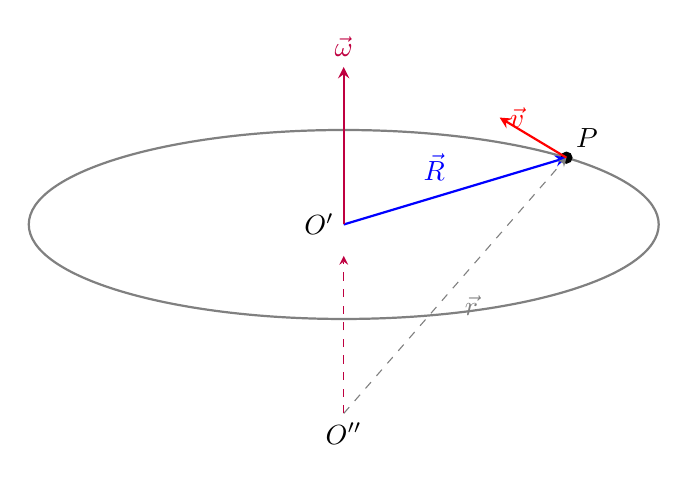
\begin{tikzpicture}[scale=2, >=stealth]

  % Елипса вместо окръжност
  \draw[gray, thick] (0,0) ellipse [x radius=2, y radius=0.6];

  % Център O'
  \coordinate (O') at (0,0);
  \node[left] at (O') {$O'$};

  % Точка P върху окръжността
  \def\angle{45}
  \def\rx{2}
  \def\ry{0.6}
  \coordinate (P) at ({\rx*cos(\angle)},{\ry*sin(\angle)});
  \filldraw[black] (P) circle (1pt) node[above right] {$P$};

  % Радиус-вектор R
  \draw[->, thick, blue] (O') -- (P) node[midway, above left] {$\vec{R}$};

  % Вектор скорост (перпендикулярен на R в равнината на диска)
  \coordinate (V) at ({-0.6*sin(\angle)},{0.6*0.6*cos(\angle)});
  \draw[->, thick, red] (P) -- ++(V) node[right] {$\vec{v}$};

  % Вектор ω (извън равнината)
  \draw[->, thick, purple] (O') -- +(0,1) node[above] {$\vec{\omega}$};

  % Допълнителен център O''
  \coordinate (O'') at (0,-1.2);
  \node[below] at (O'') {$O''$};

  % Радиус-вектор r (от O'' до P)
  \draw[->, gray, dashed] (O'') -- (P) node[midway, below right] {$\vec{r}$};

  % ω от O'' също (за да се подчертае същата посока)
  \draw[->, dashed, purple] (O'') -- +(0,1);



\end{tikzpicture}

Нека разглеждаме вектор $\vec{w}(t)$ с начало $O'$, перпенидкулярен на равнината с големина $|\vec{w}|=|\alpha'|$ както е на фигурата, където $\alpha$ е ъгълът който образува материалната точка $P$ .
Векторът $w$ образува дясна тройка числа, такава че: $\vec v = \vec w \times \vec R$
Дефиниранят по този начин $\vec w(t)$ се нарича \textbf{ъглова скорост}
Ако върху направлението на $\vec w $ избера която и да е друга точка например $O''$ спрямо която радиус-векторът е $\vec r$, скоростта добива вида:

$$\vec v= \vec w \times \vec r$$
\begin{proof}
	$$\vec w \times \vec r = \vec w \times (\vec{O'O''}+\vec R) = \vec w \times \vec{O'O''} + \vec w \times \vec R = \vec w \times \vec R$$

	
\end{proof}
Тъй като, $\vec{O'O''}$ и $\vec w$ са колинеарни

\subsection{Площна скорост}
\dfn{Площна скорост}{Площната скорост описва колко площ помита радиус-векторът \( \vec{r} \), свързващ дадено тяло с фиксирана точка (напр. център на въртене), за единица време.
Площна скорост \( \vec{\sigma} \) се дефинира като:

\[
\vec{\sigma} = \frac{1}{2} \vec{r} \times \vec{v}
\]}
\begin{proof}
	За малък ъгъл \( d\theta \) за време \( dt \), тялото изминава дъга и „помита“ малък триъгълник с площ:

\[
dS = \frac{1}{2} r^2 d\theta
\]

Тогава:

\[
\frac{dS}{dt} = \frac{1}{2} r^2 \frac{d\theta}{dt} = \frac{1}{2} r^2 \omega
\]

Или векторно:

\[
\vec{\sigma} = \frac{1}{2} \vec{r} \times \vec{v}
\]
\end{proof}


\nt{Свойства на площната скорост:\begin{itemize}
    \item \( \vec{\sigma} \) е константен при централни сили (напр. при гравитация) — това е т.нар. втори закон на Кеплер.
    \item Големината:
    \[
    |\vec{\sigma}| = \frac{1}{2} r v \sin \theta = \frac{1}{2} r v \quad \text{(ако ъгълът между } \vec{r} \text{ и } \vec{v} \text{ е } 90^\circ)
    \]
    \item За кръгово движение:
    \[
    |\vec{\sigma}| = \frac{1}{2} r^2 \omega
    \]
\end{itemize}}


\chapter{Динамика на материална точка}

\section{Основни видове сили. Принципи на Нютон. Количество на движение.}
\subsection{Основни видове сили}
В механиката разглеждаме два вида сили: \begin{itemize}
    \item Гравитационна сила
    \item Електрична сила
    \subitem триене
    \subitem реакция на опората
    \subitem сила на опън
    \subitem еластична сила
\end{itemize}
Всяка една от тези сили и нейните закони ще бъде разгледана по-подробно по-нататък.

\subsection{Принципи на Нютон}

Динамиката е науката занимаваща се с движението на телата във връзка с причините, които го предизвикват и променят.
Първото твърдение на Динамиката, така наречения Първи принцип на Нютон.
\clm{Първи принцип на Нютон}{}{Едно тяло запазва състоянието си на покой или праволинейно и равномерно движение, докато външна сила не го изведе от това положение}
\nt{Важно е да се отбележи, че стриктна дефиниция за "сила" \medspace не притежаваме, най-точната дефиниця която имаме благодарение на опита на човечеството е: Мярка за взаимодействията на телата.
Как се извършва това взаимодействие, какъв е неговия носител и други подобни въпроси не сме способни да отговорим, но за изучаването на Динамиката не е и нужно, тъй като се занимаваме с следсвята на силите, а не с причините.}
\mprop{}{В първя принцип на Нютон се съдържат две твърдения:\begin{itemize}
    \item На всички тела е присъщо свойството инертност
    \item Съществуват инерциални отправни системи $K$
\end{itemize}}
\clm{Втори приницп на Нютон}{}{Вторият принцип гласи, че: 
\begin{equation}\vec F = m\vec a\end{equation} където $\vec F$ е равнодействащата сила на тялото. 
}
\nt{Понеже масата е винаги положителна $\Rightarrow$ ускорението на тялото и равнодействаща сила винаги имат една и съща посока}
\clm{Трети принцип на Нютон}{}{За всяка сила, съществува друга равна по големина и противоположна по посока:
$$\vec F_1 = -\vec F_2$$}
Да отбележим, че двете сили не се уравновесяват защото имат различни приложни точки.
\subsection{Количество движение}
Във физиката всяко тяло с маса, което се движи, притежава инерция. Но когато се опитваме да оценим не просто дали дадено тяло е склонно да се съпротивлява на ускорение (инерция), а колко движение „носи“ със себе си, тогава въвеждаме понятието количество на движение.

Това е фундаментна величина в механиката, чрез която можем да разбираме взаимодействията между телата и всичко това е директно свързано с втория закон на Нютон.
\dfn{}{Количеството на движение (или импулс) на материална точка с маса $m$, движеща се със скорост $\vec{v}$, е:
$$\vec p=m\vec v$$ }
Тази величина може да се използва за да изразим втория закон на Нютон по друг еквивалентен начин:
$$\vec F=\dot{\vec{p}}$$
\nt{За система от материални точки общият импулс на системата се дава под \begin{itemize}
    \item $\sum_{i=1}^{n}m_i\vec v_i$
    \item Ако системата обаче има обща маса $M$ и център на масите с векторан скорост $\vec{v}_C$: $\vec{P}=M\vec{v}_C$
\end{itemize}}
\section{Сила на тежестта. Движение в полето на силата на тежестта без съпротивление и
при отчитане на съпротивлението на средата.}

Гравитационно поле е невидимо, но основно силово поле, което обкръжава всички маси и привлича други маси към себе си. Това е ключово за разбирането на движението на обектите в близост до планета или друго небесно тяло.


\subsubsection{Свободно падане и ускорение}
Феноменът на свободно падане се наблюдава, когато обектът е подложен само на гравитацията, без да действат други външни сили, като въздушно съпротивление или триене.

\textbf{Ускорение при свободно падане}: Обектите при свободно падане близо до Земята преживяват ускорение от около $9.8 \, \text{m/s}^2$ надолу. Това показва, че скоростта на обекта се увеличава с около $9.8$ метра в секунда за всяка изминала секунда на падане.
\dfn{Сила на тежестта}{Използвайки втория приницп на Нютон с земното успорение получаваме дефиницята за сила на тежестта:$$\vec F=m\vec g$$}
\subsection{Движение в полето на силата на тежестта без съпротивление}
При падане без сила на триене можем да ползваме втория приницп на Нютон заедно за да опишем движението на тялото:

\ex{Падане на тяло без триене}{Нека приемем, че тялото се движи само по остта $z$, тогава $\vec F = m\vec a \rightarrow F_z=ma_z$, щом няма триене само сила на тежестта участва: $$\vec G = m\vec a = m \ddot{z}(t)$$ $$m\ddot{z}(t)=-mg$$ }
\subsection{Движение със съпротивление}
\ex{Падане на тяло с триене}{Щом имаме триене втория приницп ще съдържа и триене на стокс $\vec F_R$ и ще има вида:$$m\ddot{z}(t)=-mg-\beta \dot{z}(t)$$
Това е Нехомогенно ОДУ което ни дава за $z(t)$ (Да се провери от читателя!!)$$z(t)=\frac{g}{\gamma}(\frac{1}{\gamma}(1-e^{-\gamma t})+t)$$ Където $\gamma = -\frac{\beta}{m}$}
\newpage
\section{Еластична сила. Движение в полето на еластична сила при отсъствие на
съпротивление. Фазови портрети}
\subsection{Закон на Хук}
Ако разтегнем пружина ще забележим, че необходимата за разтягането външна сила $\vec F$ нараства при увеличаването на деформацията $x$ на пружината. 
Съгласно 3тия принцип на Нютон, пружината противодейства със сила $\vec F_e$. Оптино е установено големината на тази сила.
\dfn{Еластична сила}{Еластичната сила, упражнявана от идеална пружина, се описва от закона на Хук:
\[
\vec{F}_e = -k \vec{x},
\]
където $k$ е коефициентът на еластичност, а $\vec{x}$ — отклонението от равновесното положение.}
\nt{Важно е да кажем, че при големи отклонения закона на Хук не е валиден и е нужно да включим втори порядъци на $x$}
\subsection{Движение без съпротивление}
Движението на маса $m$, прикрепена към пружина, при липса на съпротивление се описва чрез:
\[
m \ddot{x} + kx = 0.
\]
Това е линейно хомогенно уравнение с константни коефициенти, чието общо решение е (\textbf{Да се провери!}):
\[
x(t) = A \cos(\omega t + \phi),
\]

където $\omega = \sqrt{\frac{k}{m}}$ е ъгловата честота, $A$ — амплитудата, и $\phi$ — началната фаза.

\subsection{Фазов портрет}
Фазовият портрет представлява графика в координатите $(x, \dot{x})$ и показва траекторията на системата в пространството на състоянията.

За хармоничното трептене фазовите траектории са елипси:
\[
\frac{x^2}{A^2} + \frac{\dot{x}^2}{\omega^2 A^2} = 1.
\]
\begin{wrapfigure}{r}{0.4\textwidth}
    \centering
    \includegraphics[width=\linewidth]{image.png}
    \caption{Фазов портрет}
\end{wrapfigure}
\begin{proof}
    Започваме с уравнението на хармоничен осцилатор без съпротивление:
\[
m\ddot{x} + kx = 0 \quad \Rightarrow \quad \ddot{x} + \omega^2 x = 0, \quad \omega = \sqrt{\frac{k}{m}}
\]
Решението на това уравнение е:
\[
x(t) = A \cos(\omega t + \varphi)
\]
Производната (скоростта) е:
\[
\dot{x}(t) = -A\omega \sin(\omega t + \varphi)
\]
Изразяваме $\cos$ и $\sin$ чрез $x$ и $\dot{x}$:
\[
\cos(\omega t + \varphi) = \frac{x(t)}{A}, \quad \sin(\omega t + \varphi) = -\frac{\dot{x}(t)}{A\omega}
\]

Използваме тъждеството:
\[
\cos^2(\omega t + \varphi) + \sin^2(\omega t + \varphi) = 1
\Rightarrow \left(\frac{x}{A}\right)^2 + \left(\frac{\dot{x}}{A\omega}\right)^2 = 1
\]
Следователно фазовият портрет е:
\[
\frac{x^2}{A^2} + \frac{\dot{x}^2}{\omega^2 A^2} = 1
\]
което представлява елипса в пространството на фазовите променливи $(x, \dot{x})$.
\end{proof}

\section{Хармоничен осцилатор при наличие на съпротивление. Фазови портрети}
При наличието на съпротивление, както при свободното падане, така и в нашия случай, ще трябва да въведем затихващ елемент. Уравнението добива следващия вид:

$$m\ddot x + b \dot x +kx=0$$
$$\ddot{x}+ 2\beta\dot{x}+\omega_0^2x=0$$
\nt{$$\beta = \frac{1}{2}\frac{b}{m}, \medspace \space \omega_0=\sqrt{\frac{k}{m}}$$}
$$r^2+2\beta r+\omega_0^2=0$$
$$r_{1,2}=-\beta\pm \sqrt{\beta^2-\omega_0^2}$$
Този отговор показва, че има три вида решения:

\mprop{}{\begin{itemize}
    \item \textbf{Слабо затихване}: Характеризира се с: $\omega_0^2>\beta^2 \Rightarrow r_{1,2}=-\beta \pm i\omega_1$ Където  $\omega_1^2=\omega_0^2-\beta^2$ $$x(t)=e^{-\beta t}(C_1e^{i\omega_1 t}+C_2e^{-i\omega_1 t})$$ или в реална форма $$x(t)=Ae^{-\beta t}\cos(\omega_1 t +\delta)$$
    \item \textbf{Двоен корен }:  $\omega_0^2=\beta^2$, характеризира се със специално съотношение между силите на триене и силите на връщане. Нарича се апериодичен лимит. $$x(t)=(C_1+C_2t)e^{-\beta t}$$
    \item \textbf{Силно затихване} $\omega_0^2<\beta^2:$ $$x(t)=C_1e^{r_1 t}+C_2e^{r_2 t},$$ $r_{1,2}<0.$ Общото решение е суперпозиция  на два члена които намалят експоненциално с времето, тоест не осцилират.

\end{itemize}}

\begin{figure}[t!]
    \begin{minipage}[t]{0.20\textwidth}
        \includegraphics[width=\linewidth]{Слабо затихващ осцилатор.png}
        \caption{Слабо затихващ осцилатор}
    \end{minipage}
    \hspace{0.02\textwidth}
    \begin{minipage}[t]{0.20\textwidth}
        \includegraphics[width=\linewidth]{Апериодичен лимит.png}
        \caption{Апериодичен лимит}
    \end{minipage}
    \hspace{0.02\textwidth}
    \begin{minipage}[t]{0.20\textwidth}
        \includegraphics[width=\linewidth]{Силно затихващ осцилатор.png}
        \caption{Силно затихващ осцилатор}
    \end{minipage}
    \begin{minipage}[t]{0.20\textwidth}
        \includegraphics[width=\linewidth]{Фазов портрет слабо затихване.png}
        \caption{Фазов портрет – Слабо затихване}
    \end{minipage}
\end{figure}

\section{Трептене на хармоничен осцилатор под действието на външна хармонична сила}
\dfn{Принудителни трептения}{Принудителни осцилации са още един начин да променим задачата за хармонияния осцилатор. Такива трептения могат да бъдат характеризирани с \begin{equation}m \ddot{x} +b\dot{x} +kx=F(t)$$ или $$\ddot{x}+2\beta \dot{x}+\omega_0^2x=f(t)\end{equation} където $f=\frac{F}{m}, \space \omega_0 \medspace \text{е собствената честота на системата}$ Системата маса-пружина е под въздействието на външна сила зависеща от времето. Можем да отчетем двата случая: когато няма триене и когато има. Прост пример на външна сила е хармонична сила}
Външната сила може например да бъде зададена във вида:
\[
f(t) = \gamma \cos(\omega t).
\]

Осцилиращата маса се подлага на периодично принудително движение с външна честота \( f = \frac{\omega}{2\pi} \).

Решението на нехомогенното диференциално уравнение $(2.1)$ може да се запише във вида:
\[
x(t) = x_{\text{hom}}(C_1, C_2, t) + x_{\text{part}}(t),
\]
където общото решение на хомогенното уравнение вече е обсъдено в предишния раздел. \cor{}{Частното решение за случая на косинусоидална сила се намира с помощта на допускане:
\[
x_{\text{part}}(t) = A \cos(\omega t) + B \sin(\omega t).
\]}

Методът на променливите коефициенти може да се използва за определяне на параметрите \(A\) и \(B\), но в настоящия случай това не е необходимо. Достатъчно е да заместим израза в диференциалното уравнение:

\[
\dot{x}_{\text{part}} = -A \omega \sin(\omega t) + B \omega \cos(\omega t), \quad
\ddot{x}_{\text{part}} = -A \omega^2 \cos(\omega t) - B \omega^2 \sin(\omega t).
\]

След съпоставяне на коефициентите пред \(\cos(\omega t)\) и \(\sin(\omega t)\) получаваме:

\[
(-A\omega^2 + 2\beta B\omega + A\omega_0^2) \cos(\omega t) + 
(-B\omega^2 - 2\beta A\omega + B\omega_0^2) \sin(\omega t) = \gamma \cos(\omega t),
\]

което води до система от линейни уравнения:

\[
(-2\beta \omega)A + (\omega_0^2 - \omega^2)B = 0,
\]
\[
(\omega_0^2 - \omega^2)A + (2\beta \omega)B = \gamma.
\]

Решението е:

\[
A = \frac{\gamma(\omega_0^2 - \omega^2)}{(\omega_0^2 - \omega^2)^2 + 4\beta^2 \omega^2}, \quad
B = \frac{2\beta \gamma \omega}{(\omega_0^2 - \omega^2)^2 + 4\beta^2 \omega^2}.
\]

Често е удобно частното решение да се запише във вида:

\[
x_{\text{part}}(t) = a \cos(\omega t - \varphi),
\]
където \(a\) е амплитудата, а \(\varphi\) фазовият ъгъл. Връзките между параметрите са:

\[
a = \sqrt{A^2 + B^2}, \quad
\cos(\varphi) = \frac{A}{\sqrt{A^2 + B^2}}, \quad
\sin(\varphi) = \frac{B}{\sqrt{A^2 + B^2}}, \quad
\tan(\varphi) = \frac{B}{A}.
\]

Получаваме:

\[
a = \frac{\gamma}{\sqrt{(\omega_0^2 - \omega^2)^2 + 4\beta^2 \omega^2}}, \quad
\tan(\varphi) = \frac{2\beta \omega}{\omega_0^2 - \omega^2}.
\]

\nt{Фазата \(\varphi\) не зависи от амплитудата на външната сила.

\begin{itemize}
    \item Константите на интегриране \(C_1\) и \(C_2\) се определят от началните условия. Общото решение може да бъде доста сложно.
    \item Частното решение доминира при големи времена, ако хомогенното решение умира експоненциално:
    \[
    \lim_{t \to \infty} x(t) = x_{\text{part}}(t), \quad \text{ако } \lim_{t \to \infty} x_{\text{hom}}(t) = 0.
    \]
\end{itemize}}

\[
x_{\text{part}}(t) = a \cos(\omega t - \varphi).
\]
\clm{}{}{Тази форма показва, че движението не е в синхрон с външната сила, а я „изостава“ с фаза \(\varphi\).

В случай на принудена осцилация без затихване (\(\beta = 0\)), частното решение е:
\[
a = \frac{\gamma}{|\omega_0^2 - \omega^2|}, \quad \varphi = 0.
\]}
\nt{Интересно е да се забележи, че при $\omega \approx \omega_0$ амплитудата може да придобие много големи стойности, този феномен се нарича \textbf{Резонанс}}
Общото решение тогава е суперпозиция на два хармонични сигнала:

\[
x(t) = a_0 \cos(\omega_0 t - \delta_0) + a \cos(\omega t).
\]

Константите \(a_0\) и \(\delta_0\) се определят от началните условия. \ex{Определяне на константите}{Ако \(x(0) = 0\), \(\dot{x}(0) = 0\), получаваме:

\[
a_0 \cos(\delta_0) + a = 0, \quad
a_0 \omega_0 \sin(\delta_0) = 0,
\]

откъдето следва:
\[
\delta_0 = 0, \quad a_0 = -a.
\]

Следователно крайното решение е:

\[
x(t) = a \left( \cos(\omega t) - \cos(\omega_0 t) \right).
\]}
\section{Импулс на материална точка и момент на импулса. Закони за тяхното запазване.
Пълен импулс и момент на импулса за система от материални точки и закон за
запазването им.}



\dfn{}{Импулсът на материална точка, наричан още количество на движение, е векторна физична величина, дефинирана като произведението на масата на тялото и неговата скорост:

\[
\vec{p} =m \vec{v}
\]}



Импулсът характеризира „количеството движение“, което тялото носи.

\subsection{Закон за запазване на импулса}

Съгласно втория закон на Нютон:


$$m\frac{d\vec{v}}{dt} = \vec{F}\Rightarrow \frac{d\vec{p}}{dt} = \vec{F}$$

Когато върху системата не действа външна сила (или сумата от външните сили е нула), то \(\vec{F}_{\text{рез}} = 0\) и получаваме:

\[
\frac{d\vec{p}}{dt} = 0 \Rightarrow \vec{p} = \text{const}.
\]

Това е \textbf{законът за запазване на импулса}: В затворена система (без външни сили) сумарният импулс остава постоянен.

\subsection{Момент на импулса}

Моментът на импулса на материална точка спрямо определена точка \( O \) е дефиниран чрез векторното произведение:

\[
\vec{L} = \vec{r} \times \vec{p} = \vec{r} \times (m\vec{v}),
\]

където:
\begin{itemize}
    \item \( \vec{r} \) е радиус-векторът от точката \( O \) до материалната точка,
    \item \( \vec{L} \) — момент на импулса [kg·m²/s].
\end{itemize}
\newpage
\subsection{Закон за запазване на момента на импулса}

Производната на момента на импулса по време е равна на момента на външната сила (въртящ момент):

\[
\frac{d\vec{L}}{dt} = \vec{M} = \vec{r} \times \vec{F}.
\]
\begin{proof}
    Умножаваме векторно двете страни на втория закон на Нютон
    \begin{equation}\vec{r}\times m \frac{d\vec{v}}{dt}=\vec{r} \times \vec{F}
    \end{equation}
    $$\vec{r}\times m \frac{d\vec{v}}{dt} = \frac{d}{dt}(\vec{r} \times m\vec{v})-\frac{d\vec{r}}{dt}\times m \frac{d\vec{r}}{dt}=\frac{d}{dt}(\vec{r} \times m\vec{v})=\frac{d}{dt}(\vec{r}\times \vec{p})$$
    Тогава уравнението $(2.2)$ има вида \begin{equation}\frac{d}{dt}(\vec{r}\times \vec{p})= \vec{r}\times \vec{F}\end{equation}
    \dfn{Момент на импулса}{Величината $\vec{r}\times \vec{p}$ се нарича\textbf{момент на импулса $\vec{L}$}. }
\dfn{Момент на сила}{$\vec{r}\times \vec{F}$  се нарича \textbf{момент на сила $\vec M$}}
Тогава уравнението $(2.3)$ ще има вида: \begin{equation}
    \frac{d\vec{L}}{dt}=\vec{M}
\end{equation}
\end{proof}

Ако \( \vec{M} = 0 \), тогава:

\[
\frac{d\vec{L}}{dt} = 0 \Rightarrow \vec{L} = \text{const} \Rightarrow \vec{L}=\vec{L_0}
\]

\thm{Закон за запазване на момента на импулса}{При липса на външни въртящи моменти, моментът на импулса на една точка или система остава постоянен.}
\nt{Условието $\vec{M}=0$ може да се получи при 3 различни случая: 
\begin{itemize}
    \item Ако силата е равна на нула
    \item Ако радиус-векторът е равен на нула
    \item Ако силата $\vec{F}$ и радиус-векторът $\vec{r}$ са колинеарни
\end{itemize}
Първите два случая са тривиални. Остава третия: Силата и радиус-векторът могат да са постоянно колинеарни, само ако силата има директриса, минаваща през началото $O$. (Това не е проблем, защото изборът на начало на координатната система е съвсем произволен и можем да го вземем там където ни е удобно) Силите които изпълняват това условие се наричат \textbf{централни сили}}

\subsection{Система от $N$ на брой материални точки}

Нека имаме система от \( N \) материални точки с маси \( m_i \), скорости \( \vec{v}_i \), и външни и вътрешни сили \( \vec{F}_{\text{вън}}, \vec{F}_{\text{вътр}} \).
Валидни са следните дефиниции:
\newline
\newline
\textbf{Пълната маса:}
 $M=\sum_{i=1}^{N}m_i$
 \newline
 \newline
\textbf{Позиция на центъра на масата:}
 $R=\frac{1}{R}\sum_{i}^{}m_i\vec{r_i}$
 \newline
 \newline
\textbf{Скоростта на центъра на масата:}
 $\vec{V}=\dot{\vec{R}}=\frac{1}{M}\sum_{i}^{}m_i\vec{v_i}$
 \newline\newline
\textbf{Сумарният импулс е:}
$\vec{P} = \sum_{i=1}^N m_i \vec{v}_i=\sum_{i}^{}\vec{p_i}$
\newline
\newline
\textbf{Позицията на материална точка спряма центъра на масите:}
$\vec{r'_i}=\vec{r_i}-\vec{R}$



\thm{Закон за импулса на $N$ на брой материални точки}{\begin{equation}\dot{\vec{P}}=\vec{F}_{\text{вън}}\end{equation}}
\nt{Оставя се като упражнение на читателя да докаже, че само външните сили допринасят към промяната на импулса.}
Импулсът на системата се запазва ако сумата на външните сили е равна на 0 за $\forall$ $t$:

\begin{equation}
    \sum_k\vec{F_k}=0\rightarrow \dot{\vec{P}}=0 \rightarrow \vec{P}=const
\end{equation}


\subsection{Общ момент на импулса}

Общият момент на импулса спрямо точка \( O \) е:

\begin{equation}
\vec{L} = \sum_{i=1}^N \vec{r}_i \times m_i \vec{v}_i.
\end{equation}

\begin{equation}
\frac{d\vec{L}}{dt} = \sum_{i=1}^N \vec{r}_i \times \vec{F}_i^{\text{вън}} = \vec{M}.
\end{equation}

\nt{Ако \( \vec{M} = 0 \), то \( \vec{L} = \text{const} \). Законът за импулсът е изключително полезен инструмент за разглеждането на механични системи, обаче често се използва заедно с принципът за енергиите, което ме води до следващата точка}

\section{Кинетична и потенциална енергия. Закон за запазване на пълната механична
енергия. Потенциали на силата на тежестта, на еластичната сила, на Нютоновата
сила и Кулоновата сила.}
\subsection{Кинетична и потенциална енергия}

Ако умножим уравнение $(2.1)$ в диференциална форма с $\vec{v}=\frac{d\vec{r}}{dt}$ Ще получим:
\begin{equation}
    d\frac{mv^2}{2}=\vec{F}\cdot d\vec{r}
\end{equation}
\dfn{Кинетична енергия}{Величината $\frac{mv^2}{2}$ наричаме кинетична енергия и ще я бележим с $T$ }
\dfn{Елементарна работа}{Величината $\vec{F}\cdot d\vec{r}$ се нарича елементарна работа и ще я означим с $d'A$.}
\nt{Примът е поставен за да бележи, че тя не е пълен диференциал на някаква функция $A$, а само достатъчно малка величина}
Тогава с нашите означение имаме \begin{equation}
    dT=d'A
\end{equation}
Бихме могли да получим допълнителна информация ако интегрираме този израз, но това има свойте трудност тъй като $d'A$ не е пълен диференциал. \newline Нека означим с $M_1$ съвкупонстта от информация за положението  и скоростта в някакъв момент $t=t_1$, а с $M_2$ същата информация за момент $t=t_2>t_1$
Сега ако искаме да интегрираме ще успеем само лявата страна тъй като представлява пълен диференциал и:
\begin{equation}\int_{M_1}^{M_2}dT=T(M_2)-T(M_1)\end{equation}. \newline 
НО пресмятането на дясната част:\begin{equation}\int_{M_1}^{M_2}d'A=\int_{M_1}^{M_2}\vec{F}(t,\vec{r}, \vec{v})\cdot d\vec{r}\end{equation} би изисквало да знаем през какви състояние минава точката от $M_1$ до $M_2$ и как става това, тоест да познаваме закона за движение на точката, което обесмислия нуждата да пресмятаме интеграла.
\newline За това ни трябват такъв клас сили, за които можем  да пресметнем $(2.13)$ без нужда от допълнителни данни за движението.
\cor{}{Нека разгледаме клас сили които зависият само от мястото}
\begin{equation}
    \int_{r_1}^{r_2}\vec{F}(\vec{r}).d\vec{r}=
\end{equation}
\begin{equation}
    \int_{(x_1,y_1,z_1)}^{x_2,y_2,z_2}[X(x,y,z)dx+Y(x,y,z)dy+Z(x,y,z)dz]
\end{equation}
\nt{Сега вместо да трябва да знаем целят закон за движението на точката е достатъчно да знаем траектрорията на точката, но въпреки всичко продължава да обесмисля смятането на интеграла $(2,13)$ \newline
Особен интерес представляват сили, които зависият само от мястото, за които подинтегралният израз в $(2.13$) се превръща в пълен диференциал на някаква функция $V$.
\newline Такива сили се наричат \textbf{консервативни сили} }
\newpage
\cor{Функция на сили}{За да е изпълнено трябва да съществъва функция $V(x,y,z)$ за която:
\begin{equation}X(x,y,z)=\frac{\partial V}{\partial x}; \medspace Y(x,y,z)=\frac{\partial V}{\partial y}; \medspace Z(x,y,z)=\frac{\partial V}{\partial z}. \end{equation}}
Тогава ще получим\begin{equation}\int_{r_1}^{r_2}\vec{F}\cdot d\vec{r}=\int_{M_1}^{M_2}dV=V(M_2)-V(M_1)\end{equation}
Ние често обаче ще ползваме \begin{equation*}
    U(x,y,z)=-V 
\end{equation*}
\nt{Тази функция я наричаме \textbf{потенциал} и описва величината \textbf{потенциална енергия}}
Тоест: Ако съществува $U(x,y,z)$, че \begin{equation}
    -\text{grad}U=\vec{F}
\end{equation}
Уравнението $(2.11)$ има вида:
\begin{equation}
    d(T+U)=0
\end{equation}
След интегриране получаваме 
\dfn{ЗЗМЕ}{Законът за запазване на механичната енергията гласи, че Механичната енергия се запазва при консервативни сили:\begin{equation}
    T(M_1)+U(M_1)=T(M_2)+U(M_2) \Rightarrow T+U=E = \text{const}
\end{equation} Където $E$ е \textbf{пълната механична енергия}}
\nt{Интересен въпрос е дали механичната енергията ще се запази ако силите са неконсервативни. Отговорът е \textbf{НЕ}, но това не е в противоречие с общия закон във физиката, че енергията се запазва, защото макар и механичната енергия да не се запазва към нея се прибавят друг вид енергии в които може да се трансформира механичната енергия чрез извършване на работа или обменяне на топлина и се получава резултат съгласно закона за запазване на енергията.}
\qs{Условиe за същестуване на потенциал}{Тук представям пред читателя упражнениe което ще му помогне да зарбере природата на този материал.\begin{itemize}
    \item Докажате, че необходимото и достатъчно условие да може да се пресметне $(2.14)$ без нужда от допълнителна информация за движението е силата да е такава, че:\begin{equation}
        \vec \nabla \times \vec{F}=0
    \end{equation}
    
\end{itemize}\textit{Подсказка}: Ако интегралът $(2.14)$ взет за произволна крива ви даде една и съща стойност, то тогава незнанието на траекторията му не е проблем.
}\newpage
\subsection{Потенциали при различни сили}
Благодарение на $(2.18)$  можем да пресметнем какъв ще е потенциала за различни видове сили.
\qs{Докажете потенциалите на при различни сили}{\begin{itemize}
    \item Докажете, че потенциалната енергия при сила на тежестта е: \begin{equation}
    U(z)=mgz
    \end{equation}
    \item Докажете, че при Сила на Хук: \begin{equation}
        U(x)=\frac{kx^2}{2}
    \end{equation}
    \item При Гравитационна сила:\begin{equation}
        U(r)=-G\frac{Mm}{r}
    \end{equation}
    \item Кулонова сила(Знакът ще зависи от зарядите): \begin{equation}
        U(r)=\frac{1}{4\pi \varepsilon_0}\cdot\frac{q_1q_2}{r}
    \end{equation}
\end{itemize}
}
\chapter{Динамика на системи от материални точки}
\section{Задача за двете тела. Център на масите. Редукция на двусчастичната задача към едночастична. Система център на масите}


Редица физически задачи, включително гравитационното и електростатичното взаимодействие, могат да бъдат сведени до т.нар. \textbf{двучастична задача} — система от две материални точки, взаимодействащи чрез централна сила, пропорционална на някаква функция на разстоянието между тях.

\subsection{Описание на системата}
\begin{wrapfigure}{l}{0.45\textwidth}
  \centering
  \vspace{-10pt}
  \begin{tikzpicture}[scale=2, thick]
  % Coordinates
  \coordinate (O) at (0,0);
  \coordinate (x1) at (2,1);
  \coordinate (x2) at (1,2);
  
  % Vectors to particles
  \draw[->, thick, olive] (O) -- (x1) node[midway, below right] {$\vec{r}_1$};
  \draw[->, thick, olive] (O) -- (x2) node[midway, below left] {$\vec{r}_2$};
  
  % Relative vector
  \draw[->, thick, purple] (x1) -- (x2) node[midway, above] {$\vec{r}$};

  % Barycenter (center of mass)
  \coordinate (R) at ($(x1)!0.5!(x2)$);
  \filldraw[white] (R) circle (0.05);
  \draw[->, thick, violet] (O) -- (R) node[midway, below] {$\vec{R}$};

  % Particles
  \shade[ball color=blue!40] (x1) circle (0.15) node[left=6pt, red!80!black] {\large $m_1$};
  \shade[ball color=blue!60] (x2) circle (0.18) node[right=6pt, red!80!black] {\large $m_2$};



  % Origin
  \filldraw (O) circle (0.05) node[below right] {$O$};

\end{tikzpicture}
 \vspace{-10pt}
\end{wrapfigure}
Да въведем две тела с маси $m_1$ и $m_2$, с радиус-вектори спрямо инерциална отправна система:

\[
\vec{r}_1(t), \quad \vec{r}_2(t)
\]

Телата си взаимодействат чрез централна сила $\vec{F}_{12} = -\vec{F}_{21}$, насочена по вектора $\vec{r} = \vec{r}_1 - \vec{r}_2$.

\subsection{Уравнения на движение}


Съгласно втория закон на Нютон:

\[
m_1 \ddot{\vec{r}}_1 = \vec{F}_{12}, \qquad m_2 \ddot{\vec{r}}_2 = \vec{F}_{21} = -\vec{F}_{12}
\]

Сумираме двете уравнения:

\[
m_1 \ddot{\vec{r}}_1 + m_2 \ddot{\vec{r}}_2 = 0
\]

Въвеждаме радиус-вектора на центъра на масите:

\[
\vec{R} = \frac{m_1 \vec{r}_1 + m_2 \vec{r}_2}{m_1 + m_2}
\]

Диференцирайки два пъти:

\[
\ddot{\vec{R}} = \frac{m_1 \ddot{\vec{r}}_1 + m_2 \ddot{\vec{r}}_2}{m_1 + m_2} = 0
\]

Следователно, ако няма външни сили, центърът на масите се движи праволинейно и равномерно.

\subsection{Относително движение и редуцирана маса}

Да въведем относителния радиус-вектор:

\[
\vec{r} = \vec{r}_1 - \vec{r}_2
\]

Тогава:

\[
\ddot{\vec{r}} = \ddot{\vec{r}}_1 - \ddot{\vec{r}}_2 = \frac{\vec{F}_{12}}{m_1} + \frac{\vec{F}_{12}}{m_2} = \vec{F}_{12} \left( \frac{1}{m_1} + \frac{1}{m_2} \right)
\]

Въвеждаме \textbf{редуцирана маса}:

\[
\mu = \frac{m_1 m_2}{m_1 + m_2}
\]

\dfn{Редуцирана маса- приведена маса}{Редуцираната маса е математически трик, който позволява да сведем задача с две взаимодействуващи тела до задача с едно „въображаемо“ тяло, което се движи под действието на същата сила, но спрямо центъра на масите.\newline \textbf{Физически смисъл}\newline Тя е масата на една въображаема частица, която се движи по същия начин, както относителното движение между двете реални частици. Тоест: \begin{itemize}
    \item Преминаваме от описанието с векторите $\vec{r}_1$ и $\vec{r}_2$

    \item Към описание с центъра на масите $\vec{R}$ и относителния вектор $\vec{r} = \vec{r}_1 - \vec{r}_2$

    \item И редуцираната маса $\mu$ се използва в уравнението на движението за $\vec{r}$:
    
\end{itemize}}

и получаваме:

\[
\mu \ddot{\vec{r}} = \vec{F}_{12}(\vec{r})
\]

Това е уравнение на движение на \textbf{една частица с маса $\mu$}, движеща се под действието на централна сила.
\nt{След като сме намерили $\vec{R}$ и $\vec{r}$ можем да намерим първоначалните траектроии:
\[
\begin{cases}
\vec{r_1}(t)=\vec{R}(t)+\frac{m_2}{m_1+m_2}\vec{r}(t) \\
\vec{r_2}(t)=\vec{R}(t)-\frac{m_1}{m_1+m_2}\vec{r}(t)
\end{cases}
\]}
\subsection{Редукция към едночастична задача}

Системата от две тела с маси $m_1$ и $m_2$ е еквивалентна на:

\begin{itemize}
  \item Движение на точка с маса $m_1 + m_2$ и радиус-вектор $\vec{R}$ (център на масите);
  \item Движение на точка с маса $\mu$ и радиус-вектор $\vec{r}$, описващ относителното движение.
\end{itemize}

\clm{}{}{Движението на двете тела винаги лежът върху равнина спрямо един с друг}
Оставям го като задача за читателя да го докаже. 
\newline

\textit{Подсказка:} Използвайте изученото до сега за момент на импулса
\newpage

\section{Кеплерова задача. Траектории при различни енергии. Вектор на Лаплас-Рунге-Ленц}
\subsection{Кеплерова задача}
\dfn{Кеплерова задача}{
Кеплеровата задача разглежда движението на планетите около Слънцето или, в по-общ смисъл, движението на тяло с маса $m$ в централно гравитационно поле, създадено от тяло с маса $M$. Решенията на Кеплеровата задача описват траекториите на телата, които се движат под действието на централна сила, обратно пропорционална на квадрата на разстоянието.
}

\subsubsection{Уравнение на движението}

\dfn{Уравнение на движението}{
Движението на планета с маса $m_P$ под действието на гравитационната сила на Слънцето с маса $M$ се описва от векторното уравнение:
\[
m_P\ddot{\vec{r}} = -G\frac{M m_P}{r^3} \vec{r}
\]
където $G$ е гравитационната константа, а $\vec{r}$ е радиус-векторът от Слънцето до планетата.
}

\nt{
Масата на планетата може да се съкрати, показвайки, че орбитите не зависят от конкретната маса. Например, Земята би се движила по същата орбита като Венера, ако бъде поставена на нейната орбита с подходящите начални условия.
}

\subsubsection{Закони за запазване и оптимални координати}

\cor{Запазване на момента на импулса}{
Тъй като гравитационната сила е централна, моментът на импулса се запазва:
\[
\vec{L} = m_P \vec{r} \times \vec{v} = \text{const}
\]
Това означава, че движението се осъществява в равнина, определена от началните стойности $\vec{r}(0)$ и $\vec{v}(0)$. Ето защо полярните координати са най-подходящи за описание на движението.
}

В полярни координати векторното уравнение на движение се разлага на:
\[
a_r = \ddot{r} - r\dot{\varphi}^2 = -G \frac{M}{r^2}
\]
\[
a_{\varphi} = r\ddot{\varphi} + 2\dot{r}\dot{\varphi} = 0
\]

\cor{Закон на площите}{
Второто уравнение изразява закона за запазване на момента на импулса (закона на площите):
\[
r^2(t)\dot{\varphi}(t) = A = \text{const}
\]
където константата $A$ се определя от началните условия:
\[
A = r^2_0\dot{\varphi}_0 = \frac{l_0}{m_P}
\]
$\varphi(t)$ може да се определи чрез разделяне на променливите:
\[
\varphi(t)-\varphi_0=\int_0^t \frac{A}{r(t')^2}dt'
\]
}

\subsubsection{Интеграли на движението}

\cor{Запазване на енергията}{
Тъй като силата е консервативна, енергията също се запазва:
\[
\frac{m_P}{2}v^2 - G\frac{m_P M}{r} = E_0
\]
където $v^2 = \dot{r}^2 + r^2\dot{\varphi}^2$.
}

Радиалното диференциално уравнение, което трябва да се реши, е:
\[
\frac{1}{2}\dot{r}^2 + \frac{1}{2}\frac{A^2}{r^2} - G\frac{M}{r} = B = \frac{E_0}{m_P}
\]
\[
t=\pm \int_{r_0}^r \frac{dr'}{[2B+2G\frac{M}{r'}-\frac{A^2}{r'^2}]^{1/2}}
\]
\nt{Знакът трябва да бъде избран, така че $t=t(r)$ да е монотонно растяща функция. Проблемът на този интеграл е, че не може да се реши по аналитичен начин.}

Вместо да търсим директно функциите $r(t)$ и $\varphi(t)$, можем да определим траекторията като функция $r(\varphi)$. Използвайки верижното правило:
\[
\dot{r} = \frac{dr}{d\varphi}\dot{\varphi} = \frac{A}{r^2}\frac{dr}{d\varphi}
\]
и замествайки в израза за енергията, получаваме:
\[
\frac{1}{2}\frac{A^2}{r^4}\left(\frac{dr}{d\varphi}\right)^2 + \frac{1}{2}\frac{A^2}{r^2} - G\frac{M}{r} = B
\]
След преобразуване:
\[
\frac{dr}{d\varphi} = \pm\frac{r^2}{A}\left[2B + \frac{2G M}{r} - \frac{A^2}{r^2}\right]^{1/2}
\]
Разделянето на променливите дава:
\[
\varphi(r) - \varphi_0 = \pm\int_{r_0}^{r} \frac{A\,dr}{r^2\left[2B + \frac{2G M}{r} - \frac{A^2}{r^2}\right]^{1/2}}
\]
Този интеграл може да се пресметне чрез заместването $s = 1/r$, което води до:
\[
\varphi(s) - \varphi_0 = \mp\int_{s_0}^{s} \frac{A\,ds}{\left[2B + 2G Ms - A^2s^2\right]^{1/2}}
\]
\nt{Примитивната функция на този интеграл е (има го в стандартни таблици за интеграли):
\[
\varphi(s) - \varphi_0 = \pm\left[\arcsin\left(\frac{-A^2s + G M}{[G^2M^2 + 2A^2B]^{1/2}}\right)\right]_{s_0}^{s}
\]
}

\qs{Гранични условия}{
За удобство, избираме долната граница на интеграла $s_0$ така, че радиус-векторът и векторът на скоростта да са перпендикулярни в пресечната точка на $x$-оста и траекторията. Такива точки се характеризират с $dr/d\varphi = 0$, което води до:
\[
\frac{1}{2}A^2s_0^2-GMs_0=B
\]
Оставя се като задача на читателя да провери, че след намирането на корен на това квадратно уравнение може да се види, че долната граница на интеграла е $\varphi_0 = 0 \space \text{или}\space \pi$.
}

И решавайки спрямо $\frac{1}{r}$:
\[
\frac{A^2}{GM}\frac{1}{r}=1\pm \left[1+\frac{2A^2B}{G^2M^2}\right]^{1/2}\cos\varphi
\]

Окончателно, уравнението на траекторията в полярни координати е:
\[
\frac{p}{r} = 1 \pm e\cos\varphi
\]
където параметрите $p$ и $\varepsilon$ са свързани с константите $A$ и $B$:
\[
p = \frac{A^2}{G M} = \frac{l_0^2}{G m_P^2 M}
\]
\[
e = \left[1 + \frac{2A^2B}{G^2M^2}\right]^{1/2} = \left[1 + \frac{2l_0^2E_0}{G^2m_P^3M^2}\right]^{1/2}
\]

\subsection{Траектория при различни енергии}

\cor{Конични сечения}{
Уравнението $\frac{p}{r} = 1 \pm e\cos\varphi$ описва коничните сечения (кръг, елипса, парабола или хипербола), като координатната система е избрана така, че началото ѝ съвпада с единия фокус.

Видът на траекторията зависи от стойността на числовия ексцентрицитет $e$, който същевременно зависи от енергията:
}



\qs{Да се докаже}{
\begin{itemize}
    \item $e = 0$ (Кръгова орбита): $E_0 = -\frac{G^2M^2}{2L^2}$
    \item $0 < e < 1$ (Елиптична орбита): $E_0(\text{кръг}) < E_0 < 0$
    \item $e = 1$ (Параболична орбита): $E_0 = 0$
    \item $e > 1$ (Хиперболична орбита): $E_0 > 0$
\end{itemize}}
\nt{
- Най-ниската възможна енергия съответства на кръгова орбита.
- За енергии между минималната стойност и нула съществуват две точки на обръщане (перихелий и афелий), което съответства на елиптична орбита.
- При $E_0 = 0$ (парабола) има две квази-точки на обръщане: една близо до Слънцето, другата в безкрайност.
- При $E_0 > 0$ (хипербола) има само една точка на обръщане в близост до Слънцето.
}

\subsection{Вектор на Лаплас-Рунге-Ленц}

\dfn{Вектор на Лаплас-Рунге-Ленц}{
Векторът на Лаплас-Рунге-Ленц е особен интеграл на движението в Кеплеровата задача, който се проявява само при сили, обратно пропорционални на квадрата на разстоянието. Той се дефинира като:
\[
\vec{A} = \vec{p} \times \vec{L} - m_P G M\hat{r}
\]
или еквивалентно:
\[
\vec{A} = m_P\vec{v} \times (\vec{r} \times \vec{v}) - m_P G M\frac{\vec{r}}{r}
\]
където:
\begin{itemize}
    \item $\vec{p} = m_P\vec{v}$ е импулсът на частицата
    \item $\vec{L} = \vec{r} \times \vec{p}$ е моментът на импулса
    \item $\hat{r} = \frac{\vec{r}}{r}$ е единичен вектор по посока на радиус-вектора
\end{itemize}
}

\nt{
\textbf{Геометрична интерпретация:} Векторът $\vec{A}$ е насочен от централното тяло към перицентъра на орбитата (най-близката точка от траекторията до централното тяло). Големината на вектора е свързана с ексцентрицитета на орбитата:
\[
A = m_P G M e
\]
\textbf{Връзка с формата и ориентацията на орбитата:} Запазването на вектора $\vec{A}$ гарантира, че формата и ориентацията на орбитата са постоянни във времето. Това е директно следствие от първия закон на Кеплер (планетите се движат по елипси, в единия фокус на които се намира Слънцето).
}

\cor{Уравнение на траекторията чрез $\vec{A}$}{
Скаларното произведение на $\vec{A}$ и $\vec{r}$ дава:
\[
\vec{A} \cdot \vec{r} = (\vec{p} \times \vec{L}) \cdot \vec{r} - m_P G M r
\]
Имайки предвид, че $(\vec{p} \times \vec{L}) \cdot \vec{r} = (\vec{r} \times \vec{p}) \cdot \vec{L} = \vec{L} \cdot \vec{L} = L^2$, получаваме:
\[
\vec{A} \cdot \vec{r} = L^2 - m_P G M r
\]
От друга страна, използвайки дефиницията $A = m_PG M e$, можем да запишем:
\[
\vec{A} \cdot \vec{r} = A r \cos\varphi = m_PG M e r\cos\varphi
\]
Приравнявайки двата израза:
\[
m_P G M e r\cos\varphi = L^2 - m_PG M r
\]
След преобразуване получаваме:
\[
r = \frac{L^2/m_PG M}{1 + e\cos\varphi} = \frac{p}{1 + e\cos\varphi}
\]
което е точно уравнението на коничното сечение в полярни координати.
}

\qs{Проверка на запазването на $\vec{A}$}{
Да се докаже, че векторът на Лаплас-Рунге-Ленц е интеграл на движението, т.е. $\frac{d\vec{A}}{dt} = 0$.
\[
\frac{d\vec{A}}{dt} = \frac{d}{dt}(\vec{p} \times \vec{L} - m_PG M\hat{r}) = 0
\]
\textit{Подсказка:} Използвайте, че $\frac{d\vec{p}}{dt} = \vec{F}$, $\frac{d\vec{L}}{dt} = 0$ и изразете $\frac{d\hat{r}}{dt}$.
}

% ...existing code...
\section{Система с връзки, видове връзки. Уравнения на Лагранж от първи ред. Примери.}
\dfn{Несвободна система от материални точки}{Тя се нарича несвободна система от материални точки, ако е налице връзка(ограничение) между координатите и скоростите на материалните точки. В най-общия вид изглеждат по следния начин: \begin{equation} f(\vec{r}_\alpha, \space \vec{v}_\alpha, \space t)\ge 0 \end{equation}}
Както и при връзките на една материална точка, връзките от тип (3.1) могат да бъдат класифицирани:

\begin{itemize}
    \item \textbf{Едностранни или неудуржащи}
    \subitem Такива връзки наричаме, ако (3.1) е пълно неравенство, тоест: $f(\vec{r}_\alpha, \space \vec{v}_\alpha, \space t)> 0$.
    \item \textbf{Двустранни или удържащи}
    \subitem Такива връзки наричаме, ако (3.1) е пълно равенство, тоест: $f(\vec{r}_\alpha, \space \vec{v}_\alpha, \space t)= 0$.
    \item \textbf{Нестационарни}
    \subitem Ако връзките съдържат явна зависимост от времето
    \item \textbf{Стационарни}
    \subitem Ако връзките не съдържат явна зависимост от времето
    \item \textbf{Диференциални}
    \subitem Ако връките съдържат поне една от скоростите
    \item \textbf{Крайни или геометрични}
    \subitem Ако връзките не съдържат скоростите
\end{itemize}
\nt{Част от диференциалните връзки могат да бъдат интеграирани. Съвкупността от тези връзки и крайните се нарича: \textbf{Холономни връзки}. \newline \newline
Често ще разглеждаме връзки които са \textbf{двустранни, стационарни и крайни}\begin{equation} f(x_\alpha, \space y_\alpha, \space z_\alpha)=0\end{equation}\begin{equation}f(\vec{r})=0\end{equation} }

\subsection{Реакция на връзката и сили на реакция}
Нека разгледаме случай на една материална точка с маса $m$, върху която действа сила $\vec{F}$ и се движи под въздействието на двустранна стационарна връзка $f(\vec{r})=0$. Диференцирайки връзката по времето получаваме:
\begin{equation}
\frac{df}{dt} = \nabla f \cdot \frac{d\vec{r}}{dt} = \nabla f \cdot \vec{v} = 0
\end{equation}

От това следва, че $\nabla f \perp \vec{v}$, т.е. скоростта е перпендикулярна на градиента на връзката. Движението на точката се осъществява изцяло по повърхността, определена от $f(\vec{r})=0$. 

Диференцирайки още веднъж, получаваме условие за ускорението:
\begin{equation}
\frac{d^2f}{dt^2} = \nabla f \cdot \frac{d\vec{v}}{dt} + \frac{d(\nabla f)}{dt} \cdot \vec{v} = \nabla f \cdot \vec{a} + D^2f = 0
\end{equation}
където $D^2f$ бележи израза, съдържащ втори производни на $f$.

\nt{Вторият закон на Нютон $m\vec{a} = \vec{F}$ трябва да бъде модифициран, за да отчете наличието на връзка, тъй като не всяка произволна сила $\vec{F}$ ще удовлетворява условието $\nabla f \cdot \vec{F} + mD^2f = 0$, получено след заместване.}

\dfn{Сила на реакция на връзката}{За да отчетем влиянието на връзката, добавяме допълнителна сила $\vec{R}$, наречена сила на реакция:
\begin{equation}
m\vec{a} = \vec{F} + \vec{R}
\end{equation}
Където $\vec{F}$ е резултантната на всички приложени сили (без да отчитаме връзката), а $\vec{R}$ е силата на реакция на връзката.}

Силата на реакция може да се разложи на две компоненти:
\begin{equation}
\vec{R} = \lambda\nabla f + \vec{T}
\end{equation}
Където:
\begin{itemize}
    \item $\lambda\nabla f$ - компонента, перпендикулярна на повърхността на движение (успоредна на $\nabla f$)
    \item $\vec{T}$ - компонента в равнината на движение (тангенциална компонента)
\end{itemize}
\clm{Разлагане на вектор $\vec{R}$}{}{Реално тук сме използвали, че $3n$-мерният вектор $\vec{R}$ винаги може да бъде представен като линейна комбинация на $3n$ линейно независими вектора}
\dfn{Идеална връзка}{Наричаме една връзка идеална, ако тангенциалната компонента на силата на реакция е нула: $\vec{T} = \vec{0}$. В този случай силата на реакция е винаги перпендикулярна на скоростта и не извършва работа.}

\subsection{Уравнения на Лагранж от първи ред}
За идеална връзка имаме:
\begin{equation}
m\vec{a} = \vec{F} + \lambda\nabla f
\end{equation}

Заместваме това в условието за ускорението $\nabla f \cdot \vec{a} + D^2f = 0$ и получаваме:
\begin{equation}
\nabla f \cdot \frac{\vec{F} + \lambda\nabla f}{m} + D^2f = 0
\end{equation}

От това намираме множителя на Лагранж $\lambda$:
\begin{equation}
\lambda = -\frac{\nabla f \cdot \vec{F} + mD^2f}{|\nabla f|^2}
\end{equation}

\thm{Уравнения на Лагранж от първи ред}{За система от $n$ материални точки с маси $m_\alpha$ ($\alpha = 1, 2, ..., n$), свързани с $m$ стационарни връзки вида:
\begin{equation}
f_k(\vec{r}_1, \vec{r}_2, ..., \vec{r}_n) = 0, \quad k = 1, 2, ..., m
\end{equation}
уравненията на движение се записват във вида:
\begin{equation}
m_\alpha\vec{a}_\alpha = \vec{F}_\alpha + \sum_{k=1}^{r}\lambda_k\nabla_\alpha f_k, \quad \alpha = 1, 2, ..., n
\end{equation}
където $\lambda_k$ са множители на Лагранж, независещи от конкретната частица, а $\nabla_\alpha f_k$ е градиентът на $f_k$ спрямо координатите на частицата $\alpha$.}

\nt{Системата от уравнения (3.10) заедно с уравненията на връзките $f_k = 0$ образува система от $3n+m$ уравнения за $3n+m$ неизвестни: $x_\alpha(t)$, $y_\alpha(t)$, $z_\alpha(t)$ и $\lambda_k(t)$.}

\subsection{Примери}
\ex{Материална точка, движеща се по сфера}
{Нека имаме материална точка с маса $m$, движеща се по повърхността на сфера с радиус $R$ и център в началото на координатната система. Върху точката действа сила на тежестта $\vec{F} = m\vec{g}$.

Връзката се задава чрез уравнението:
\begin{equation}
f(\vec{r}) = x^2 + y^2 + z^2 - R^2 = 0
\end{equation}

Градиентът на връзката е:
\begin{equation}
\nabla f = 2(x\vec{i} + y\vec{j} + z\vec{k}) = 2\vec{r}
\end{equation}

Според уравненията на Лагранж от първи ред:
\begin{equation}
m\vec{a} = m\vec{g} + \lambda\nabla f = m\vec{g} + 2\lambda\vec{r}
\end{equation}

За да намерим $\lambda$, първо трябва да пресметнем $D^2f$:
\begin{equation}
D^2f = \frac{d(\nabla f)}{dt} \cdot \vec{v} = \frac{d(2\vec{r})}{dt} \cdot \vec{v} = 2\vec{v} \cdot \vec{v} = 2|\vec{v}|^2
\end{equation}

Следователно:
\begin{equation}
\lambda = -\frac{\nabla f \cdot \vec{F} + mD^2f}{|\nabla f|^2} = -\frac{2\vec{r} \cdot m\vec{g} + m \cdot 2|\vec{v}|^2}{|2\vec{r}|^2} = -\frac{2m\vec{r} \cdot \vec{g} + 2m|\vec{v}|^2}{4R^2}
\end{equation}

Да опростим:
\begin{equation}
\lambda = -\frac{m\vec{r} \cdot \vec{g} + m|\vec{v}|^2}{2R^2}
\end{equation}

Уравнението на движение става:
\begin{equation}
\vec{a} = \vec{g} - \frac{\vec{r} \cdot \vec{g} + |\vec{v}|^2}{R^2}\vec{r}
\end{equation}

Това е уравнението на движение на материална точка по повърхността на сфера под действие на силата на тежестта.}

\ex{Махало (математично)}{
Нека разгледаме математично махало - материална точка с маса $m$, окачена на нерастяжима нишка с дължина $l$.

Връзката се задава чрез:
\begin{equation}
f(x, y, z) = x^2 + y^2 + (z - l)^2 - l^2 = 0
\end{equation}
Което след опростяване дава:
\begin{equation}
f(x, y, z) = x^2 + y^2 + z(z - 2l) = 0
\end{equation}

Градиентът е:
\begin{equation}
\nabla f = 2x\vec{i} + 2y\vec{j} + 2(z - l)\vec{k}
\end{equation}

Силата, действаща на частицата, е силата на тежестта $\vec{F} = m\vec{g} = -mg\vec{k}$.

Според уравненията на Лагранж от първи ред:
\begin{equation}
m\vec{a} = m\vec{g} + \lambda\nabla f
\end{equation}

След заместване и решаване на системата от уравнения, получаваме диференциалното уравнение на математичното махало:
\begin{equation}
\frac{d^2\theta}{dt^2} + \frac{g}{l}\sin\theta = 0
\end{equation}
Където $\theta$ е ъгълът на отклонение от вертикалната ос.}

\ex{Частица в равнина, наклонена спрямо хоризонта}
{Нека имаме частица с маса $m$, движеща се по равнина, наклонена под ъгъл $\alpha$ спрямо хоризонта. Уравнението на равнината може да се запише като:
\begin{equation}
f(x, y, z) = z - x\tan\alpha = 0
\end{equation}

Градиентът на връзката е:
\begin{equation}
\nabla f = -\tan\alpha\vec{i} + \vec{k}
\end{equation}

Прилагайки уравненията на Лагранж от първи ред, получаваме движение на частицата по равнината под действие на силата на тежестта, като нормалната компонента от теглото се компенсира от реакцията на опората, а тангенциалната компонента предизвиква ускоряване по наклона.}



Трябва да се отбележи, че уравненията на Лагранж от първи ред работят с декартови координати, което в някои случаи може да усложни решението. За по-сложни системи често е по-удобно да се използват обобщени координати и уравнения на Лагранж от втори ред.
\newpage
\section{Принцип за виртуалната работа на Даламбер. Уравнения на Лагранж от втори род
при наличието на консервативни и неконсервативни сили.}


\subsection{Принцип за виртуалната работа на Даламбер}

\dfn{Виртуално преместване}{Малко въображаемо преместване на системата $\delta \vec{r}_\alpha$, което е съвместимо с връзките в даден момент от времето, но при което времето $t$ не се променя.}

\nt{За стационарни връзки виртуалните премествания трябва да удовлетворяват:
\begin{equation}
\sum_{\alpha=1}^{n} \nabla_\alpha f_k \cdot \delta \vec{r}_\alpha = 0, \quad k = 1, 2, ..., r
\end{equation}
където $r$ е броят на връзките.}

\dfn{Виртуална работа}{Работата, извършена от сила $\vec{F}$ при виртуално преместване $\delta \vec{r}$:
\begin{equation}
\delta A = \vec{F} \cdot \delta \vec{r}
\end{equation}}

\thm{Принцип на виртуалната работа (Принцип на Даламбер)}{За система от $n$ материални точки с маси $m_\alpha$, подложени на връзки и действащи сили $\vec{F}_\alpha$, сумата от виртуалните работи на всички приложени сили и инерционните сили е равна на нула:
\begin{equation}
\sum_{\alpha=1}^{n} (\vec{F}_\alpha - m_\alpha \vec{a}_\alpha) \cdot \delta \vec{r}_\alpha = 0
\end{equation}
за всички виртуални премествания $\delta \vec{r}_\alpha$, съвместими с връзките в системата.}

Това уравнение можем да запишем и като:
\begin{equation}
\sum_{\alpha=1}^{n} \vec{F}_\alpha \cdot \delta \vec{r}_\alpha - \sum_{\alpha=1}^{n} m_\alpha \vec{a}_\alpha \cdot \delta \vec{r}_\alpha = 0
\end{equation}

Принципът на Даламбер може да се интерпретира като обобщение на втория закон на Нютон за системи с връзки. Той гласи, че при всяко виртуално преместване, съвместимо с връзките, виртуалната работа на приложените сили заедно с инерционните сили е равна на нула.

\nt{Величините $-m_\alpha \vec{a}_\alpha$ се наричат \textbf{даламберови сили} или \textbf{сили на инерция}. Те винаги са насочени в посока, противоположна на ускорението.}

Доказателство: Нека запишем уравненията на Лагранж от първи ред:
\begin{equation}
m_\alpha \vec{a}_\alpha = \vec{F}_\alpha + \sum_{k=1}^{r} \lambda_k \nabla_\alpha f_k
\end{equation}

Преобразуваме до:
\begin{equation}
\vec{F}_\alpha - m_\alpha \vec{a}_\alpha = - \sum_{k=1}^{r} \lambda_k \nabla_\alpha f_k
\end{equation}

Умножаваме скаларно с виртуалното преместване $\delta \vec{r}_\alpha$ и сумираме по всички частици:
\begin{equation}
\sum_{\alpha=1}^{n} (\vec{F}_\alpha - m_\alpha \vec{a}_\alpha) \cdot \delta \vec{r}_\alpha = - \sum_{\alpha=1}^{n} \sum_{k=1}^{r} \lambda_k \nabla_\alpha f_k \cdot \delta \vec{r}_\alpha
\end{equation}

За виртуални премествания, съвместими с връзките, имаме:
\begin{equation}
\sum_{\alpha=1}^{n} \nabla_\alpha f_k \cdot \delta \vec{r}_\alpha = 0
\end{equation}

Следователно, дясната страна на уравнение (3.7) е нула, което доказва принципа на Даламбер.

\subsection{Обобщени координати и степени на свобода}

\dfn{Степени на свобода}{Минималният брой независими параметри, необходими за еднозначно определяне на положението на системата.}

За система от $n$ материални точки в тримерното пространство без връзки, броят на степените на свобода е $3n$. При наличие на $r$ независими холономни връзки, броят на степените на свобода става $s = 3n - r$.

\dfn{Обобщени координати}{Набор от $s$ независими параметри $q_1, q_2, ..., q_s$, които еднозначно определят положението на системата и са съвместими с връзките.}

Радиус-векторите на материалните точки могат да бъдат изразени чрез обобщените координати:
\begin{equation}
\vec{r}_\alpha = \vec{r}_\alpha(q_1, q_2, ..., q_s, t)
\end{equation}

При стационарни връзки имаме:
\begin{equation}
\vec{r}_\alpha = \vec{r}_\alpha(q_1, q_2, ..., q_s)
\end{equation}

Виртуалните премествания могат да се изразят чрез вариациите на обобщените координати:
\begin{equation}
\delta \vec{r}_\alpha = \sum_{i=1}^{s} \frac{\partial \vec{r}_\alpha}{\partial q_i} \delta q_i
\end{equation}

\subsection{Обобщени сили}

\dfn{Обобщена сила}{Величина $Q_i$, съответстваща на обобщената координата $q_i$, която се определя от условието:
\begin{equation}
\sum_{\alpha=1}^{n} \vec{F}_\alpha \cdot \delta \vec{r}_\alpha = \sum_{i=1}^{s} Q_i \delta q_i
\end{equation}}

От това следва:
\begin{equation}
Q_i = \sum_{\alpha=1}^{n} \vec{F}_\alpha \cdot \frac{\partial \vec{r}_\alpha}{\partial q_i}
\end{equation}

За консервативна система с потенциална енергия $U(q_1, q_2, ..., q_s)$, обобщените сили се изразяват като:
\begin{equation}
Q_i = -\frac{\partial U}{\partial q_i}
\end{equation}

\subsection{Кинетична енергия в обобщени координати}

Скоростта на материалната точка може да се изрази чрез обобщените координати и техните производни по времето (обобщени скорости $\dot{q}_i$):
\begin{equation}
\vec{v}_\alpha = \frac{d\vec{r}_\alpha}{dt} = \sum_{i=1}^{s} \frac{\partial \vec{r}_\alpha}{\partial q_i} \dot{q}_i + \frac{\partial \vec{r}_\alpha}{\partial t}
\end{equation}

За стационарни връзки:
\begin{equation}
\vec{v}_\alpha = \sum_{i=1}^{s} \frac{\partial \vec{r}_\alpha}{\partial q_i} \dot{q}_i
\end{equation}

Кинетичната енергия на системата в обобщени координати:
\begin{equation}
T = \sum_{\alpha=1}^{n} \frac{m_\alpha v_\alpha^2}{2} = \sum_{\alpha=1}^{n} \frac{m_\alpha}{2} \left| \sum_{i=1}^{s} \frac{\partial \vec{r}_\alpha}{\partial q_i} \dot{q}_i \right|^2
\end{equation}

При стационарни връзки кинетичната енергия може да се записати във вида:
\begin{equation}
T = \frac{1}{2} \sum_{i=1}^{s} \sum_{j=1}^{s} a_{ij} \dot{q}_i \dot{q}_j
\end{equation}
където коефициентите $a_{ij}$ са функции на обобщените координати:
\begin{equation}
a_{ij} = \sum_{\alpha=1}^{n} m_\alpha \frac{\partial \vec{r}_\alpha}{\partial q_i} \cdot \frac{\partial \vec{r}_\alpha}{\partial q_j}
\end{equation}

\nt{Важно е да се отбележи, че $a_{ij} = a_{ji}$, т.е. матрицата на коефициентите е симетрична.}

\subsection{Уравнения на Лагранж от втори род}

\thm{Уравнения на Лагранж от втори род}{За холономна механична система с $s$ степени на свобода уравненията на движение имат вида:
\begin{equation}
\frac{d}{dt} \left( \frac{\partial T}{\partial \dot{q}_i} \right) - \frac{\partial T}{\partial q_i} = Q_i, \quad i = 1, 2, ..., s
\end{equation}}

Доказателство: Нека приложим принципа на Даламбер:
\begin{equation}
\sum_{\alpha=1}^{n} (\vec{F}_\alpha - m_\alpha \vec{a}_\alpha) \cdot \delta \vec{r}_\alpha = 0
\end{equation}

Изразяваме $\delta \vec{r}_\alpha$ чрез вариациите на обобщените координати:
\begin{equation}
\sum_{\alpha=1}^{n} (\vec{F}_\alpha - m_\alpha \vec{a}_\alpha) \cdot \sum_{i=1}^{s} \frac{\partial \vec{r}_\alpha}{\partial q_i} \delta q_i = 0
\end{equation}

Разменяме реда на сумиране:
\begin{equation}
\sum_{i=1}^{s} \left[ \sum_{\alpha=1}^{n} (\vec{F}_\alpha - m_\alpha \vec{a}_\alpha) \cdot \frac{\partial \vec{r}_\alpha}{\partial q_i} \right] \delta q_i = 0
\end{equation}

Тъй като вариациите $\delta q_i$ са независими, коефициентът при всяка от тях трябва да е нула:
\begin{equation}
\sum_{\alpha=1}^{n} (\vec{F}_\alpha - m_\alpha \vec{a}_\alpha) \cdot \frac{\partial \vec{r}_\alpha}{\partial q_i} = 0
\end{equation}

или
\begin{equation}
\sum_{\alpha=1}^{n} \vec{F}_\alpha \cdot \frac{\partial \vec{r}_\alpha}{\partial q_i} = \sum_{\alpha=1}^{n} m_\alpha \vec{a}_\alpha \cdot \frac{\partial \vec{r}_\alpha}{\partial q_i}
\end{equation}

Лявата страна е обобщената сила $Q_i$. За дясната страна се използва следното съотношение:
\begin{equation}
\sum_{\alpha=1}^{n} m_\alpha \vec{a}_\alpha \cdot \frac{\partial \vec{r}_\alpha}{\partial q_i} = \frac{d}{dt} \left( \frac{\partial T}{\partial \dot{q}_i} \right) - \frac{\partial T}{\partial q_i}
\end{equation}

С това получаваме уравненията на Лагранж от втори род.

\subsection{Функция на Лагранж (Лагранжиан)}

\dfn{Функция на Лагранж (Лагранжиан)}{За консервативна система с потенциална енергия $U$, функцията на Лагранж се дефинира като разликата между кинетичната и потенциалната енергия:
\begin{equation}
L(q_1, q_2, ..., q_s, \dot{q}_1, \dot{q}_2, ..., \dot{q}_s, t) = T - U
\end{equation}}

\thm{Уравнения на Лагранж с Лагранжиан}{За консервативна система уравненията на Лагранж от втори род могат да се запишат във вида:
\begin{equation}
\frac{d}{dt} \left( \frac{\partial L}{\partial \dot{q}_i} \right) - \frac{\partial L}{\partial q_i} = 0, \quad i = 1, 2, ..., s
\end{equation}}

Това е еквивалентна форма на уравненията на Лагранж за консервативни системи, където обобщените сили могат да се изразят чрез потенциалната енергия: $Q_i = -\frac{\partial U}{\partial q_i}$.



\subsection{Свойства на уравненията на Лагранж от втори род}

\qs{Какви са основните свойства на уравненията на Лагранж от втори род?}{Уравненията на Лагранж от втори род притежават редица важни свойства, които ги правят предпочитан инструмент в теоретичната механика:}

1. \textbf{Инвариантност спрямо избора на координати}: Уравненията на Лагранж запазват вида си при произволна трансформация на обобщените координати.

2. \textbf{Естествено отчитане на връзките}: Връзките са вече отчетени в избора на обобщени координати, затова не се налага явното им включване в уравненията.

3. \textbf{Универсалност}: Приложими са за широк клас механични системи, включително такива с нестационарни връзки.

4. \textbf{Скаларност}: Работи се със скаларни величини (енергии) вместо с векторни (сили), което опростява математичния апарат.

\cor{Симетрии и закони за запазване}{Всяка симетрия в Лагранжиана води до съответен закон за запазване (теорема на Ньотер). Например:
\begin{itemize}
    \item Ако $L$ не зависи явно от координата $q_i$, то съответният обобщен импулс $p_i = \frac{\partial L}{\partial \dot{q}_i}$ се запазва.
    \item Ако $L$ не зависи явно от времето $t$, то енергията на системата $E = \sum_{i=1}^{s} \dot{q}_i \frac{\partial L}{\partial \dot{q}_i} - L$ се запазва.
\end{itemize}
Ще бъде разгледано по-подробно в следващите глави.}


\subsection{Примери}

\ex{Математично махало}{
Разглеждаме математично махало с дължина $l$ и маса $m$, подложено на гравитационно поле.

\qs{Задача}{Да се изведе диференциалното уравнение на движение на математичното махало, използвайки уравненията на Лагранж от втори род.}

\textbf{Решение:}

Избираме ъгъла на отклонение $\theta$ като обобщена координата.

Координатите на махалото са:
\begin{equation}
x = l \sin \theta, \quad y = -l \cos \theta
\end{equation}

Кинетична енергия:
\begin{equation}
T = \frac{1}{2} m v^2 = \frac{1}{2} m \left( \dot{x}^2 + \dot{y}^2 \right) = \frac{1}{2} m l^2 \dot{\theta}^2
\end{equation}

Потенциална енергия:
\begin{equation}
U = mgy = -mgl \cos \theta
\end{equation}

Лагранжиан:
\begin{equation}
L = T - U = \frac{1}{2} m l^2 \dot{\theta}^2 + mgl \cos \theta
\end{equation}

Прилагаме уравнението на Лагранж:
\begin{equation}
\frac{d}{dt} \left( \frac{\partial L}{\partial \dot{\theta}} \right) - \frac{\partial L}{\partial \theta} = 0
\end{equation}

\begin{equation}
\frac{d}{dt} \left( ml^2 \dot{\theta} \right) - (-mgl \sin \theta) = 0
\end{equation}

\begin{equation}
ml^2 \ddot{\theta} + mgl \sin \theta = 0
\end{equation}

\begin{equation}
\ddot{\theta} + \frac{g}{l} \sin \theta = 0
\end{equation}

\cor{Диференциално уравнение на махалото}{Движението на математичното махало се описва от нелинейното диференциално уравнение:
\begin{equation}
\ddot{\theta} + \frac{g}{l} \sin \theta = 0
\end{equation}
При малки ъгли на отклонение ($\sin \theta \approx \theta$), уравнението се опростява до линейно:
\begin{equation}
\ddot{\theta} + \frac{g}{l} \theta = 0
\end{equation}
Това е уравнение на хармоничен осцилатор с ъглова честота $\omega = \sqrt{\frac{g}{l}}$.}
}

\subsubsection{Движение на частица в централно поле}

\ex{Движение на частица в централно поле}{
Разглеждаме частица с маса $m$, движеща се в централно поле с потенциална енергия $U(r)$.

\qs{Задача}{Да се изведат диференциалните уравнения на движение и да се покаже, че моментът на импулса се запазва.}

\textbf{Решение:}

Избираме полярни координати $(r, \varphi)$ като обобщени координати.

Кинетична енергия:
\begin{equation}
T = \frac{1}{2} m v^2 = \frac{1}{2} m \left( \dot{r}^2 + r^2 \dot{\varphi}^2 \right)
\end{equation}

Лагранжиан:
\begin{equation}
L = T - U = \frac{1}{2} m \left( \dot{r}^2 + r^2 \dot{\varphi}^2 \right) - U(r)
\end{equation}

Уравненията на Лагранж:

За координата $r$:
\begin{equation}
\frac{d}{dt} \left( \frac{\partial L}{\partial \dot{r}} \right) - \frac{\partial L}{\partial r} = 0
\end{equation}

\begin{equation}
\frac{d}{dt} \left( m\dot{r} \right) - \left( mr\dot{\varphi}^2 - \frac{dU}{dr} \right) = 0
\end{equation}

\begin{equation}
m\ddot{r} - mr\dot{\varphi}^2 + \frac{dU}{dr} = 0
\end{equation}

За координата $\varphi$:
\begin{equation}
\frac{d}{dt} \left( \frac{\partial L}{\partial \dot{\varphi}} \right) - \frac{\partial L}{\partial \varphi} = 0
\end{equation}

\begin{equation}
\frac{d}{dt} \left( mr^2\dot{\varphi} \right) - 0 = 0
\end{equation}

\begin{equation}
\frac{d}{dt} \left( mr^2\dot{\varphi} \right) = 0
\end{equation}

\cor{Закон за запазване на момента на импулса}{Уравнението 
\begin{equation}
\frac{d}{dt} \left( mr^2\dot{\varphi} \right) = 0
\end{equation}
означава, че $mr^2\dot{\varphi} = \text{const} = L$, където $L$ е моментът на импулса. Това е математичен израз на закона за запазване на момента на импулса в централно поле и следва директно от факта, че Лагранжианът не зависи от ъгловата координата $\varphi$ (симетрия при ротация).}
}

\subsubsection{Двойно махало}

\ex{Двойно махало}{
Разглеждаме двойно махало, състоящо се от две точкови маси $m_1$ и $m_2$, свързани с нерастяжими пръчки с дължини $l_1$ и $l_2$.

\qs{Задача}{Да се състави Лагранжианът на системата и да се изведат уравненията на движение.}

\textbf{Решение:}

Избираме ъглите $\theta_1$ и $\theta_2$ като обобщени координати, където $\theta_1$ е ъгълът между първата пръчка и вертикалата, а $\theta_2$ е ъгълът между втората пръчка и вертикалата.

Координатите на първата маса:
\begin{equation}
x_1 = l_1 \sin \theta_1, \quad y_1 = -l_1 \cos \theta_1
\end{equation}

Координатите на втората маса:
\begin{equation}
x_2 = l_1 \sin \theta_1 + l_2 \sin \theta_2, \quad y_2 = -l_1 \cos \theta_1 - l_2 \cos \theta_2
\end{equation}

Скоростите:
\begin{equation}
\dot{x}_1 = l_1 \dot{\theta}_1 \cos \theta_1, \quad \dot{y}_1 = l_1 \dot{\theta}_1 \sin \theta_1
\end{equation}

\begin{equation}
\dot{x}_2 = l_1 \dot{\theta}_1 \cos \theta_1 + l_2 \dot{\theta}_2 \cos \theta_2, \quad \dot{y}_2 = l_1 \dot{\theta}_1 \sin \theta_1 + l_2 \dot{\theta}_2 \sin \theta_2
\end{equation}

Кинетична енергия:
\begin{equation}
\begin{split}
T &= \frac{1}{2}m_1(\dot{x}_1^2 + \dot{y}_1^2) + \frac{1}{2}m_2(\dot{x}_2^2 + \dot{y}_2^2) \\
&= \frac{1}{2}m_1 l_1^2 \dot{\theta}_1^2 + \frac{1}{2}m_2 \left[ l_1^2 \dot{\theta}_1^2 + l_2^2 \dot{\theta}_2^2 + 2l_1 l_2 \dot{\theta}_1 \dot{\theta}_2 \cos(\theta_1 - \theta_2) \right]
\end{split}
\end{equation}

Потенциална енергия:
\begin{equation}
U = m_1 g y_1 + m_2 g y_2 = -m_1 g l_1 \cos \theta_1 - m_2 g (l_1 \cos \theta_1 + l_2 \cos \theta_2)
\end{equation}

Лагранжиан:
\begin{equation}
\begin{split}
L &= T - U \\
&= \frac{1}{2}m_1 l_1^2 \dot{\theta}_1^2 + \frac{1}{2}m_2 \left[ l_1^2 \dot{\theta}_1^2 + l_2^2 \dot{\theta}_2^2 + 2l_1 l_2 \dot{\theta}_1 \dot{\theta}_2 \cos(\theta_1 - \theta_2) \right] \\
&+ m_1 g l_1 \cos \theta_1 + m_2 g (l_1 \cos \theta_1 + l_2 \cos \theta_2)
\end{split}
\end{equation}

Применяме уравненията на Лагранж за $\theta_1$ и $\theta_2$ и след определени алгебрични преобразувания получаваме система от две нелинейни диференциални уравнения от втори ред:

\begin{equation}
\begin{split}
(m_1 + m_2)l_1^2 \ddot{\theta}_1 + m_2 l_1 l_2 \ddot{\theta}_2 \cos(\theta_1 - \theta_2) + \\
m_2 l_1 l_2 \dot{\theta}_2^2 \sin(\theta_1 - \theta_2) + (m_1 + m_2)g l_1 \sin \theta_1 = 0
\end{split}
\end{equation}

\begin{equation}
m_2 l_2^2 \ddot{\theta}_2 + m_2 l_1 l_2 \ddot{\theta}_1 \cos(\theta_1 - \theta_2) - \\
m_2 l_1 l_2 \dot{\theta}_1^2 \sin(\theta_1 - \theta_2) + m_2 g l_2 \sin \theta_2 = 0
\end{equation}

\cor{Сложност на системата}{Системата уравнения за двойното махало е нелинейна и не може да бъде решена аналитично в общия случай. При определени начални условия движението на двойното махало става хаотично, което го прави класически пример за хаотична система в механиката. Това показва как сравнително проста механична система може да проявява сложно непредсказуемо поведение.}
}
\section{Вариационен принцип на Хамилтън. Физически смисъл на вариационния принцип}

\qs{Какво представлява вариационният принцип на Хамилтън.}{Вариационният принцип на Хамилтън е един от най-фундаменталните принципи в теоретичната физика. Той формулира движението на механичните системи чрез екстремизиране на определен интеграл - \textbf{Действието}. Този принцип не само дава алтернативна формулировка на законите на механиката, но разкрива и дълбок физически смисъл за природата на движението.}

\subsection{Дефиниция на действието и принципа на Хамилтън}

\dfn{Действие }{За механична система с Лагранжиан $L(q_i, \dot{q}_i, t)$, действието $S$ е функционал, дефиниран като:
\begin{equation}
S[q_i(t)] = \int_{t_1}^{t_2} L(q_i, \dot{q}_i, t) \, dt
\end{equation}
където интегрирането се извършва по време между два фиксирани момента $t_1$ и $t_2$.}
\textbf{Функционал} е оператор който взима функция и връща число
\nt{Действието е \textbf{функционал} - това означава, че то зависи от цялата функция $q_i(t)$, а не само от нейните стойности в отделни точки. С други думи, действието е "функция от функции".}

\thm{Принцип на най-малкото действие (Принцип на Хамилтън)}{Реалното движение на механичната система между два фиксирани момента $t_1$ и $t_2$ и между фиксирани крайни положения $q_i(t_1) = q_i^{(1)}$ и $q_i(t_2) = q_i^{(2)}$ е такова, че действието $S[q_i(t)]$ има екстремална стойност (обикновено минимум).

Математически това се записва като:
\begin{equation}
\delta S = \delta \int_{t_1}^{t_2} L(q_i, \dot{q}_i, t) \, dt = 0
\end{equation}
за произволни вариации $\delta q_i(t)$, които изчезват в крайните точки: $\delta q_i(t_1) = \delta q_i(t_2) = 0$.}

\subsection{Извеждане на уравненията на Лагранж от принципа на Хамилтън}

\ex{Извеждане на уравненията на Лагранж от вариационния принцип}{
\qs{Задача}{Да се покаже как от принципа на Хамилтън следват уравненията на Лагранж от втори род.}

\textbf{Решение:}

Започваме с условието за екстремум на действието:
\begin{equation}
\delta S = \delta \int_{t_1}^{t_2} L(q_i, \dot{q}_i, t) \, dt = 0
\end{equation}

Вариацията може да се внесе под интеграла:
\begin{equation}
\delta S = \int_{t_1}^{t_2} \delta L \, dt = \int_{t_1}^{t_2} \left( \frac{\partial L}{\partial q_i} \delta q_i + \frac{\partial L}{\partial \dot{q}_i} \delta \dot{q}_i \right) dt = 0
\end{equation}

Забележаваме, че $\delta \dot{q}_i = \frac{d}{dt}(\delta q_i)$, тъй като вариацията и диференцирането по времето са комутативни операции.

Прилагаме интегриране по части за втория член:
\begin{equation}
\int_{t_1}^{t_2} \frac{\partial L}{\partial \dot{q}_i} \delta \dot{q}_i \, dt = \int_{t_1}^{t_2} \frac{\partial L}{\partial \dot{q}_i} \frac{d}{dt}(\delta q_i) \, dt
\end{equation}

\begin{equation}
= \left[ \frac{\partial L}{\partial \dot{q}_i} \delta q_i \right]_{t_1}^{t_2} - \int_{t_1}^{t_2} \frac{d}{dt}\left(\frac{\partial L}{\partial \dot{q}_i}\right) \delta q_i \, dt
\end{equation}

Тъй като $\delta q_i(t_1) = \delta q_i(t_2) = 0$, първият член изчезва:
\begin{equation}
\int_{t_1}^{t_2} \frac{\partial L}{\partial \dot{q}_i} \delta \dot{q}_i \, dt = - \int_{t_1}^{t_2} \frac{d}{dt}\left(\frac{\partial L}{\partial \dot{q}_i}\right) \delta q_i \, dt
\end{equation}

Заместваме обратно в израза за $\delta S$:
\begin{equation}
\delta S = \int_{t_1}^{t_2} \left[ \frac{\partial L}{\partial q_i} - \frac{d}{dt}\left(\frac{\partial L}{\partial \dot{q}_i}\right) \right] \delta q_i \, dt = 0
\end{equation}

Тъй като вариациите $\delta q_i$ са произволни и независими, интегралът може да бъде нула само ако:
\begin{equation}
\frac{d}{dt}\left(\frac{\partial L}{\partial \dot{q}_i}\right) - \frac{\partial L}{\partial q_i} = 0
\end{equation}

\cor{Еквивалентност на формулировките}{Принципът на Хамилтън и уравненията на Лагранж от втори род са напълно еквивалентни формулировки на законите на класическата механика. Всяка от тях може да бъде извлечена от другата. Това показва дълбоката връзка между диференциалните принципи (уравнения на Лагранж) и интегралните принципи (принцип на Хамилтън) в механиката.}
}

\subsection{Физически смисъл на вариационния принцип}

\qs{Какъв е физическият смисъл на принципа на най-малкото действие?}{Принципът на най-малкото действие има няколко важни физически интерпретации, които разкриват фундаментални аспекти на природата на физическите процеси:}


\subsubsection{3. Симетрии и закони за запазване}

Вариационният принцип естествено води до връзката между симетрии и закони за запазване (теорема на Ньотер). Ако действието е инвариантно спрямо определена трансформация, това води до съответен закон за запазване.

\ex{Примери за симетрии и запазване}{
\begin{itemize}
    \item \textbf{Хомогенност на времето}: Ако $L$ не зависи явно от $t$, то енергията се запазва
    \item \textbf{Хомогенност на пространството}: Ако $L$ е инвариантен спрямо транслации, то импулсът се запазва
    \item \textbf{Изотропност на пространството}: Ако $L$ е инвариантен спрямо ротации, то моментът на импулса се запазва
\end{itemize}
}

\subsection{Обобщения и приложения}

\subsubsection{Принцип на стационарното действие}

\nt{По-точно трябва да говорим за принцип на \textbf{стационарното} действие, а не задължително на минималното. В общия случай действието има екстремум (може да бъде минимум, максимум или седлова точка), но не задължително минимум.}

\dfn{Стационарно действие}{Реалното движение на системата съответства на стационарна точка на функционала за действието:
\begin{equation}
\frac{\delta S}{\delta q_i} = 0
\end{equation}
Това означава, че първата вариация на действието изчезва.}



\subsection{Модификации за неконсервативни системи}

За системи с неконсервативни сили принципът на Хамилтън може да бъде модифициран по няколко начина, тук ще дам пример за само един:

\subsubsection{1. Обобщен принцип на Хамилтън}

За системи с обобщени сили $Q_i^{(nc)}$, които не произлизат от потенциал:
\begin{equation}
\delta \int_{t_1}^{t_2} L \, dt + \int_{t_1}^{t_2} Q_i^{(nc)} \delta q_i \, dt = 0
\end{equation}

\

\subsection{Алтернативни формулировки}

\ex{Принцип на Мопертуи (Принцип на най-малкото действие в ограничена форма)}{
За консервативни системи с постоянна енергия $E$ може да се формулира принцип за минимизиране на съкратеното действие:
\begin{equation}
\delta \int p_i \, dq_i = 0
\end{equation}
където $p_i = \frac{\partial T}{\partial \dot{q}_i}$ са обобщените импулси, а интегрирането се извършва по пространствената траектория при фиксирана енергия.

Този принцип е особено полезен в геометричната оптика и при изучаване на движението в потенциални полета.
}


\cor{Предимства на вариационния подход}{
\begin{itemize}
    \item \textbf{Ковариантност}: Уравненията запазват формата си при произволни трансформации на координатите
    \item \textbf{Систематичност}: Предоставя единен подход за различни типове механични системи
    \item \textbf{Връзка със симетриите}: Естествено води до откриване на закони за запазване
    \item \textbf{Обобщимост}: Лесно се обобщава за релативистки системи, теория на полетата и квантова механика
\end{itemize}
}

\newpage
\section{Обобщени потенциали. Обобщен потенциал на електромагнитните сили}

\subsection{Въведение в концепцията за обобщени потенциали}

\qs{Защо имаме нужда от обобщени потенциали?}{В класическата механика работим с консервативни сили, които могат да се представят като градиент на скаларен потенциал $V$. Обаче в природата съществуват сили, като електромагнитните, които не могат да се опишат единствено чрез скаларен потенциал. Тези сили зависят не само от положението, но и от скоростта на частицата.}

\dfn{Обобщен потенциал}{Функция $U(q_i, \dot{q}_i, t)$, която зависи от обобщените координати, техните производни по времето и времето, от която могат да се получат обобщените сили чрез:
$$Q_i = -\frac{\partial U}{\partial q_i} + \frac{d}{dt}\frac{\partial U}{\partial \dot{q}_i}$$}

\subsection{Мотивация и развитие на концепцията}

\qs{Как стигаме до понятието за обобщен потенциал?} {Нека разгледаме уравненията на Лагранж:}

$$\frac{d}{dt}\frac{\partial L}{\partial \dot{q}_i} - \frac{\partial L}{\partial q_i} = Q_i$$

където $Q_i$ са обобщените сили. За консервативни сили имаме $Q_i = -\frac{\partial V}{\partial q_i}$, където $V$ е потенциалната енергия.

\nt{Ако съществува функция $U(q_i, \dot{q}_i, t)$ такава, че обобщените сили могат да се представят във вида:
$$Q_i = -\frac{\partial U}{\partial q_i} + \frac{d}{dt}\frac{\partial U}{\partial \dot{q}_i}$$
то тази функция наричаме обобщен потенциал.}

При наличие на обобщен потенциал, уравненията на Лагранж приемат вида:

$$\frac{d}{dt}\frac{\partial}{\partial \dot{q}_i}(T - U) - \frac{\partial}{\partial q_i}(T - U) = 0$$


където $T$ е кинетичната енергия, а $U$ е обобщеният потенциал.

\subsection{Електромагнитни сили и векторен потенциал}

\qs{Как електромагнитните сили се вписват в тази схема?} {Електромагнитните сили върху заредена частица се описват от силата на Лоренц:}

$$\vec{F} = q(\vec{E} + \vec{v} \times \vec{B})$$

където $q$ е зарядът на частицата, $\vec{E}$ е електричното поле, $\vec{v}$ е скоростта и $\vec{B}$ е магнитното поле.

\dfn{Електромагнитни потенциали}{Електричното и магнитното поле могат да се представят чрез скаларен потенциал $\phi$ и векторен потенциал $\vec{A}$:
$$\vec{E} = -\nabla \phi - \frac{\partial \vec{A}}{\partial t}$$
$$\vec{B} = \nabla \times \vec{A}$$}

\subsection{Извеждане на обобщения потенциал за електромагнитни сили}

\ex{Извеждане на обобщения потенциал}{Нека разгледаме частица със заряд $q$ в електромагнитно поле. Силата на Лоренц в компонентен вид е:

$$F_x = q\left(E_x + \dot{y}B_z - \dot{z}B_y\right)$$

Използвайки израженията за полетата чрез потенциалите:
$$E_x = -\frac{\partial \phi}{\partial x} - \frac{\partial A_x}{\partial t}$$
$$B_y = \frac{\partial A_x}{\partial z} - \frac{\partial A_z}{\partial x}$$
$$B_z = \frac{\partial A_y}{\partial x} - \frac{\partial A_x}{\partial y}$$

След заместване и преобразувания получаваме:
$$F_x = -q\frac{\partial}{\partial x}(\phi - \vec{v} \cdot \vec{A}) + q\frac{d}{dt}\frac{\partial}{\partial \dot{x}}(\vec{v} \cdot \vec{A})$$}

\thm{Обобщен потенциал на електромагнитните сили}{За частица със заряд $q$ в електромагнитно поле, обобщеният потенциал е:
$$U = q(\phi - \vec{v} \cdot \vec{A}) = q\phi - q\sum_{i=1}^{3} \dot{x}_i A_i$$}

\subsection{Лагранжиан на заредена частица в електромагнитно поле}

\cor{Лагранжиан в електромагнитно поле}{За частица с маса $m$ и заряд $q$ в електромагнитно поле:
$$L = T - U = \frac{1}{2}m\vec{v}^2 - q\phi + q\vec{v} \cdot \vec{A}$$}

В декартови координати:
$$L = \frac{1}{2}m(\dot{x}^2 + \dot{y}^2 + \dot{z}^2) - q\phi + q(\dot{x}A_x + \dot{y}A_y + \dot{z}A_z)$$

\subsection{Проверка на уравненията на Лагранж}

\ex{Проверка за x-компонентата}{Нека проверим, че уравненията на Лагранж дават правилната сила:

$$\frac{\partial L}{\partial \dot{x}} = m\dot{x} + qA_x$$

$$\frac{d}{dt}\frac{\partial L}{\partial \dot{x}} = m\ddot{x} + q\frac{dA_x}{dt} = m\ddot{x} + q\left(\frac{\partial A_x}{\partial t} + \sum_j \dot{x}_j \frac{\partial A_x}{\partial x_j}\right)$$

$$\frac{\partial L}{\partial x} = -q\frac{\partial \phi}{\partial x} + q\sum_j \dot{x}_j \frac{\partial A_j}{\partial x}$$

Уравнението на Лагранж $\frac{d}{dt}\frac{\partial L}{\partial \dot{x}} - \frac{\partial L}{\partial x} = 0$ дава:

$$m\ddot{x} = q\left(\frac{\partial \phi}{\partial x} - \frac{\partial A_x}{\partial t} - \sum_j \dot{x}_j \frac{\partial A_x}{\partial x_j} + \sum_j \dot{x}_j \frac{\partial A_j}{\partial x}\right)$$

След преобразувания това се свежда до силата на Лоренц.}


\subsection{Канонични импулси в електромагнитно поле}

\dfn{Канонични импулси}{В присъствието на електромагнитно поле, каноничните импулси са:
$$p_i = \frac{\partial L}{\partial \dot{q}_i}$$}

За декартови координати:
$$p_x = m\dot{x} + qA_x$$
$$p_y = m\dot{y} + qA_y$$  
$$p_z = m\dot{z} + qA_z$$

\nt{Каноничните импулси се различават от механичните импулси $m\vec{v}$ с добавката $q\vec{A}$. Тази добавка отразява взаимодействието на заредената частица с векторния потенциал. \newline 
Този резултат е в ядрото на квантовата теория за заредена частица в магнитно поле, където се оказва, че обобщеният импулс съответства на диференциалния оператор $-i\hbar\nabla$ (където $\hbar$ е редуцираната константа на Планк), така че квантовият аналог на механичния импулс $m\vec{v}$ е операторът $-i\hbar\nabla - q\vec{A}$}

\qs{Докажете, че тези два лангранжяна дават еднакви уравнения за движението}{Нека $F = F(q_1, \dots, q_n)$ бъде произволна функция на обобщените координати $q_1, \dots, q_n$ на система с Лагранжиан $L(q_i, \dots, q_n, \dot{q}_1, \dots, \dot{q}_n, t)$. Докажете, че двата Лагранжиана — $L$ и $L_1 = L + \frac{dF}{dt}$ — водят до точно същите уравнения на движение.}

\textbf{Това е свързано с калибровачни преобразувания, но е задължително да е запознат читателя с тях за да реши задачата}
\section{Теорема на Ньотер. Примери}
\nt{Преди да започна бих искал да кажа, че теоремата на Ньотер е изключително важна, и се препоръчва на читателя да отдели повече време за да ч научи, за това препоръчвам един доста пълен анализ на теоремата с примери: 
\href{https://profoundphysics.com/noethers-theorem-a-complete-guide/}{пълния наръчник за теоремата на Ньотер}.}
\subsection{Увод и мотивация}

\qs{Защо законите за запазване са толкова важни в физиката?} {До сега сме видели няколко закона за запазване - на енергията, импулса и момента на импулса. Тези закони не са случайни, а са свързани със симетриите на физическите системи.}

\qs{Какво е симетрия в физиката?} {Симетрия означава, че физическата система изглежда и се държи по същия начин при определени преобразувания. Например, законите на физиката са еднакви във всички точки от пространството (хомогенност на пространството).}

\dfn{Симетрия на Лагранжиана}{Казваме, че Лагранжианът $L(q_i, \dot{q}_i, t)$ притежава симетрия, ако съществува преобразуване на координатите, при което той остава инвариантен (неизменен).}

\subsection{Формулировка на теоремата на Ньотер}

\thm{Теорема на Ньотер}{За всяка непрекъсната симетрия на Лагранжиана съществува съответен запазващ се интеграл на движението.}

По-точно, ако Лагранжианът е инвариантен относно едно-параметрично преобразуване:
$$q_i \rightarrow q_i + \epsilon f_i(q_j, \dot{q}_j, t)$$

където $\epsilon$ е малък параметър, то съществува запазваща се величина:
$$I = \sum_i \frac{\partial L}{\partial \dot{q}_i} f_i(q_j, \dot{q}_j, t) = \text{const}$$

\subsection{Извеждане на теоремата}

\ex{Извеждане на основната формула}{Нека разгледаме едно-параметрично преобразуване:
$$q_i \rightarrow q_i' = q_i + \epsilon f_i(q_j, \dot{q}_j, t)$$

При това преобразуване скоростите стават:
$$\dot{q}_i' = \dot{q}_i + \epsilon \frac{df_i}{dt}$$

Ако Лагранжианът е инвариантен, то:
$$L(q_i', \dot{q}_i', t) = L(q_i, \dot{q}_i, t)$$

Разлагайки в ред на Тейлор до първи ред по $\epsilon$:
$$L + \epsilon \sum_i \left(\frac{\partial L}{\partial q_i} f_i + \frac{\partial L}{\partial \dot{q}_i} \frac{df_i}{dt}\right) = L$$

Следователно:
$$\sum_i \left(\frac{\partial L}{\partial q_i} f_i + \frac{\partial L}{\partial \dot{q}_i} \frac{df_i}{dt}\right) = 0$$}

Използвайки уравненията на Лагранж $\frac{d}{dt}\frac{\partial L}{\partial \dot{q}_i} = \frac{\partial L}{\partial q_i}$:

$$\sum_i \left(\frac{d}{dt}\frac{\partial L}{\partial \dot{q}_i} f_i + \frac{\partial L}{\partial \dot{q}_i} \frac{df_i}{dt}\right) = 0$$

$$\frac{d}{dt}\left(\sum_i \frac{\partial L}{\partial \dot{q}_i} f_i\right) = 0$$

\cor{Запазваща се величина}{Това означава, че величината:
$$I = \sum_i \frac{\partial L}{\partial \dot{q}_i} f_i = \sum_i p_i f_i$$
се запазва по време, където $p_i = \frac{\partial L}{\partial \dot{q}_i}$ са обобщените импулси.}

\subsection{Пример 1: Хомогенност на пространството и запазване на импулса}

\ex{Транслационна симетрия}{Разгледайме система от частици с Лагранжиан:
$$L = \sum_{\alpha} \frac{1}{2}m_{\alpha}\dot{\vec{r}}_{\alpha}^2 - V(\vec{r}_1, \vec{r}_2, ...)$$

Ако потенциалът $V$ зависи само от относителните разстояния между частиците, то системата е инвариантна относно транслации в пространството.

Преобразуването е:
$$\vec{r}_{\alpha} \rightarrow \vec{r}_{\alpha} + \epsilon \vec{n}$$

където $\vec{n}$ е единичен вектор в дадена посока.

За x-компонентата: $f_{\alpha x} = 1$ за всички частици.

Запазващата се величина е:
$$I_x = \sum_{\alpha} \frac{\partial L}{\partial \dot{x}_{\alpha}} \cdot 1 = \sum_{\alpha} m_{\alpha}\dot{x}_{\alpha} = P_x$$}

\cor{Запазване на импулса}{Хомогенността на пространството води до запазване на пълния импулс на системата:
$$\vec{P} = \sum_{\alpha} m_{\alpha}\vec{v}_{\alpha} = \text{const}$$}

\subsection{Пример 2: Изотропност на пространството и запазване на момента на импулса}

\ex{Ротационна симетрия}{Ако системата е инвариантна относно завъртания около дадена ос (например z-оста), то преобразуването е:
$$x_{\alpha} \rightarrow x_{\alpha} - \epsilon y_{\alpha}$$
$$y_{\alpha} \rightarrow y_{\alpha} + \epsilon x_{\alpha}$$
$$z_{\alpha} \rightarrow z_{\alpha}$$

Това означава: $f_{\alpha x} = -y_{\alpha}$, $f_{\alpha y} = x_{\alpha}$, $f_{\alpha z} = 0$.

Запазващата се величина е:
$$I_z = \sum_{\alpha} \left(m_{\alpha}\dot{x}_{\alpha}(-y_{\alpha}) + m_{\alpha}\dot{y}_{\alpha}x_{\alpha}\right)$$
$$I_z = \sum_{\alpha} m_{\alpha}(x_{\alpha}\dot{y}_{\alpha} - y_{\alpha}\dot{x}_{\alpha}) = L_z$$}

\cor{Запазване на момента на импулса}{Изотропността на пространството води до запазване на момента на импулса:
$$\vec{L} = \sum_{\alpha} \vec{r}_{\alpha} \times m_{\alpha}\vec{v}_{\alpha} = \text{const}$$}



\subsection{Пример 3: Хомогенност на времето и закон за запазване на енергията}
Ще се спрем  малко повече върху този анализ тъй като е важен за Хамилтоновата механика.

\ex{Времева симетрия}{Да разгледаме Лагранжиан $L(q_i, \dot{q}_i, t)$, когато времето напредва лангранжяна се променя както защото $t$ се променя, но и $q_i$ и $\dot{q}_i$ се променят. Тогава  от верижното правило:
\begin{equation}
\frac{dL}{dt} = \sum_i \left(\frac{\partial L}{\partial q_i} \dot{q}_i + \frac{\partial L}{\partial \dot{q}_i} \ddot{q}_i\right) + \frac{\partial L}{\partial t}.
\end{equation}
Сега заради уравнението на Лагранж, можем да заменим производната на първата сума с:
\begin{equation}
    \frac{\partial L}{\partial q_i}=\frac{d}{dt}\frac{\partial L}{\partial \dot{q_i}}= \frac{d}{dt}p_i=\dot{p}_i 
\end{equation}
А втората прозиводна е просто обобщения импулс $p_i$ и можем да запишем $(3.95)$:
\begin{equation}
    \frac{d}{dt}L=\sum_i(\dot{p}_i \dot{q}_i + p_i \ddot{q}_i) + \frac{\partial L}{\partial t} \newline 
    =\frac{d}{dt}\sum_i(p_i\dot{q}_i)+\frac{\partial L}{\partial t}.
\end{equation}

За много интересни системи Лагранжианът не зависи изрично от времето, т.е. $\frac{\partial L}{\partial t} = 0$. В този случай можем да запишем (3.97) като:
\begin{equation}
    \frac{d}{dt}L=\frac{d}{dt}\sum_i(p_i\dot{q}_i).
\end{equation}
Ако интегрираме (3.98) по време, получаваме:
\begin{equation}
    L = \sum_i p_i \dot{q}_i + C,
\end{equation}
където $C$ е константа на интегриране. Тази константа може да зависи от началните условия, но не зависи от времето.
Ако сега изразим $C$ като $H$, получаваме:
\begin{equation}
    H = \sum_i p_i \dot{q}_i - L,
\end{equation}
което е Хамилтонианът на системата.}
\nt{Ако Лагранжианът не зависи изрично от врмето $\Rightarrow$ Хамилтонианът $H$ се запазва.}

\cor{Смисъл на Хамилтонианът}{Ако обобщените координати и декартовите координати са независещи от времето: \textbf{Хамилтонианът е пълната енергия на системата}}
\begin{proof}
    \begin{equation}
    H = \sum_i p_i \dot{q}_i - L = \sum_i (m_i\dot{q}_i^2) - L = 2T-(T-U)=T+U
    \end{equation}
\end{proof}

\subsection{Обобщение}

\cor{Фундаментално значение}{Теоремата на Ньотер показва дълбоката връзка между симетриите и законите за запазване:
\begin{itemize}
\item Транслационна симетрия $\Rightarrow$ Запазване на импулса
\item Ротационна симетрия $\Rightarrow$ Запазване на момента на импулса  
\item Хомогенност на времето $\Rightarrow$ Запазване на енергията
\end{itemize}}
\newpage
\section{Обобщени импулси. Фазово пространство. Хамилтониан и канонични уравнения на Хамилтън}

\subsection{Обобщени импулси}

\qs{Как се свързват обобщените импулси с уравненията на Лагранж?}{От уравненията на Лагранж:
$$\frac{d}{dt}\left(\frac{\partial L}{\partial \dot{q}_i}\right) - \frac{\partial L}{\partial q_i} = 0$$
Но $\frac{\partial L}{\partial \dot{q}_i} = p_i$, така че:
$$\dot{p}_i = \frac{\partial L}{\partial q_i}$$}

\cor{Обобщена сила}{Това показва, че скоростта на промяна на обобщения импулс е равна на "обобщената сила" $\frac{\partial L}{\partial q_i}$.}

\thm{Закон за запазване на обобщения импулс}{Припомняме, че ако лагранжианът не зависи явно от координатата $q_i$ (т.е. $\frac{\partial L}{\partial q_i} = 0$), то съответният обобщен импулс $p_i$ се запазва: $p_i = \text{const}$.}



\cor{Физически смисъл на обобщените импулси}{Обобщените импулси не винаги имат физически смисъл на "обичайни" импулси. $p_\phi$ например е момент на импулса, не линеен импулс.}




\subsection{Фазово пространство}

\dfn{Фазово пространство}{Фазовото пространство на система с $n$ степени на свобода е $2n$-мерното пространство с координати $(q_1, q_2, ..., q_n, p_1, p_2, ..., p_n)$.}

\qs{Защо фазовото пространство е толкова важно?}{То ни позволява да представим пълното състояние на механичната система в един момент от време като една точка в това пространство. Еволюцията на системата се описва като траектория в фазовото пространство.}





\subsection{Канонични уравнения на Хамилтън}

\thm{Канонични уравнения на Хамилтън}{Движението на механична система се описва от системата от $2n$ диференциални уравнения от първи ред:
\begin{align}
\dot{q}_i &= \frac{\partial H}{\partial p_i}\\
\dot{p}_i &= -\frac{\partial H}{\partial q_i}
\end{align}
за $i = 1, 2, ..., n$.}

\begin{proof}
  Започваме от дефиницията на хамилтониана:
$$H = \sum_i p_i \dot{q}_i - L$$
Вземаме пълния диференциал:
$$dH = \sum_i \dot{q}_i dp_i + \sum_i p_i d\dot{q}_i - \sum_i \frac{\partial L}{\partial q_i} dq_i - \sum_i \frac{\partial L}{\partial \dot{q}_i} d\dot{q}_i$$
Но $\frac{\partial L}{\partial \dot{q}_i} = p_i$, така че:
$$dH = \sum_i \dot{q}_i dp_i - \sum_i \frac{\partial L}{\partial q_i} dq_i$$
От уравненията на Лагранж: $\dot{p}_i = \frac{\partial L}{\partial q_i}$, следователно:
$$dH = \sum_i \dot{q}_i dp_i - \sum_i \dot{p}_i dq_i$$
Сравнявайки с $dH = \sum_i \frac{\partial H}{\partial q_i} dq_i + \sum_i \frac{\partial H}{\partial p_i} dp_i$, получаваме каноничните уравнения.
\end{proof}
\newpage
\subsection{Примери}

\ex{Пример: Канонични уравнения за маса върху конус}{

Да разгледаме маса $m$, която е ограничена да се движи по гладка повърхност на вертикален конус, зададен от уравнението $\rho = cz$ (в цилиндрични координати $\rho, \varphi, z$ с $z > 0$), в еднородно гравитационно поле $g$ насочено вертикално надолу.

Използвайки $z$ и $\varphi$ като обобщени координати, да се съставят каноничните уравнения на Хамилтън. Да се покаже, че за всяко решение съществуват максимална и минимална височина $z_{\max}$ и $z_{\min}$, между които движението е ограничено. Да се използва този резултат, за да се опише движението на масата по конуса. Да се покаже също, че за всяка фиксирана стойност на $z > 0$ съществува решение, при което масата се движи по кръгова траектория с постоянна височина $z$.

Нека $\rho = cz$ е наложеното ограничение. Кинетичната енергия е:

\[
T = \frac{1}{2}m\left(\dot{\rho}^2 + \rho^2 \dot{\varphi}^2 + \dot{z}^2\right)
= \frac{1}{2}m\left((c^2 + 1)\dot{z}^2 + c^2 z^2 \dot{\varphi}^2\right)
\]

Потенциалната енергия е:

\[
U = mgz
\]

Обобщените импулси са:

\[
p_z = \frac{\partial T}{\partial \dot{z}} = m(c^2 + 1)\dot{z}, \qquad
p_\varphi = \frac{\partial T}{\partial \dot{\varphi}} = m c^2 z^2 \dot{\varphi}
\]

Решаваме тези изрази за $\dot{z}$ и $\dot{\varphi}$ и записваме Хамилтониана:

\[
H = \frac{p_z^2}{2m(c^2 + 1)} + \frac{p_\varphi^2}{2m c^2 z^2} + mgz
\]

Каноничните уравнения са:

\[
\dot{z} = \frac{\partial H}{\partial p_z} = \frac{p_z}{m(c^2 + 1)}, \qquad
\dot{p}_z = -\frac{\partial H}{\partial z} = \frac{p_\varphi^2}{m c^2 z^3} - mg
\]
\[
\dot{\varphi} = \frac{\partial H}{\partial p_\varphi} = \frac{p_\varphi}{m c^2 z^2}, \qquad
\dot{p}_\varphi = -\frac{\partial H}{\partial \varphi} = 0
\]

Тъй като $H$ е константа, получаваме ефективен потенциал, който води до това $z$ да бъде ограничено между $z_{\min}$ и $z_{\max}$. Движението е осцилиращо по $z$ и кръгово по $\varphi$ с постоянен ъглов момент.
}

\subsection{Запазване на енергията}

\thm{Запазване на хамилтониана}{Ако хамилтонианът не зависи явно от времето ($\frac{\partial H}{\partial t} = 0$), то той се запазва по време на движението:
$$\frac{dH}{dt} = \frac{\partial H}{\partial t} + \sum_i \left(\frac{\partial H}{\partial q_i}\dot{q}_i + \frac{\partial H}{\partial p_i}\dot{p}_i\right) = 0$$}

\begin{proof}
Използвайки каноничните уравнения:
$$\frac{dH}{dt} = \frac{\partial H}{\partial t} + \sum_i \left(\frac{\partial H}{\partial q_i} \frac{\partial H}{\partial p_i} + \frac{\partial H}{\partial p_i} \left(-\frac{\partial H}{\partial q_i}\right)\right) = \frac{\partial H}{\partial t}$$
Следователно, ако $\frac{\partial H}{\partial t} = 0$, то $\frac{dH}{dt} = 0$.
\end{proof}

\cor{Интерпретация}{За консервативни системи (без зависящи от времето сили) хамилтонианът представлява пълната механична енергия и се запазва.}
\subsection{Упражнения за читателя}
\qs{Частица подложена на централна възстановяваща сила}{Да се разгледа частица с маса $m$, движеща се в две измерения, подложена на сила $\vec{F} = -Kx\hat{x}+K\hat{y}$,
където $k$ и $K$ са положителни константи. Да се запише Хамилтонианът и уравненията на Хамилтън, като се използват $x$ и $y$ като обобщени координати. Да се решат уравненията и да се опише движението.}
\qs{Частица върху цилиндър с централна сила}{Да се разгледа частица с маса $m$, ограничена да се движи по гладък цилиндър с радиус $R$,
зададен чрез уравнението $p = R$ в цилиндрични полярни координати $(p, \theta, z)$. Частицата е подложена само на една външна сила $\vec{F} = -kr\hat{r}$, където $k$ е положителна константа, $r$ е разстоянието от началото, а $\hat{r}$ е единичен вектор, насочен навън от началото. Използвайки $z$ и $\theta$ като обобщени координати, да се намери Хамилтонианът $H$, да се запишат и решат уравненията на Хамилтън и да се опише движението}
\newpage
\chapter{Канонични трансформации}
\section{Скобки на Поасон между обобщените координати, обобщените импулси и момента на импулса}

\subsection{Въведение и мотивация}

\qs{Защо се нуждаем от скобките на Поасон?}{В хамилтоновата механика работим с канонични променливи $q_i$ и $p_i$. За да опишем еволюцията на произволна физична величина във времето, се нуждаем от алгебричен апарат, който свързва различните физични величини с хамилтониана на системата.}
Условието да бъдарт \textbf{канонични променливи} означава да удовлетворяват каноничните уравнения на Хамилтон с Хамилтониан: $\dot{q}_i = \frac{\partial H}{\partial p_i}$ и $\dot{p}_i = -\frac{\partial H}{\partial q_i}$.
\dfn{Скобки на Поасон}{За две функции $f(q,p,t)$ и $g(q,p,t)$ в фазовото пространство, скобката на Поасон се дефинира като:
$$\{f,g\} = \sum_{i=1}^{n} \left(\frac{\partial f}{\partial q_i}\frac{\partial g}{\partial p_i} - \frac{\partial f}{\partial p_i}\frac{\partial g}{\partial q_i}\right)$$
където $n$ е броят на степените на свобода на системата.}

\subsection{Основни свойства на скобките на Поасон}

\thm{Алгебрични свойства}{Скобките на Поасон притежават следните основни свойства:
\begin{enumerate}
\item \textbf{Антисиметричност:} $\{f,g\} = -\{g,f\}$
\item \textbf{Билинейност:} $\{af + bg, h\} = a\{f,h\} + b\{g,h\}$
\item \textbf{Правило на Лайбниц:} $\{fg, h\} = f\{g,h\} + \{f,h\}g$
\item \textbf{Тъждество на Якоби:} $\{f,\{g,h\}\} + \{g,\{h,f\}\} + \{h,\{f,g\}\} = 0$
\end{enumerate}}

\cor{Следствие от антисиметричността}{От антисиметричността директно следва, че $\{f,f\} = 0$ за всяка функция $f$.}

\subsection{Фундаментални скобки на Поасон}

\thm{Канонични комутационни соотношения}{Между каноничните променливи съществуват следните фундаментални скобки на Поасон:
\begin{align}
\{q_i, q_j\} &= 0 \\
\{p_i, p_j\} &= 0 \\
\{q_i, p_j\} &= \delta_{ij}
\end{align}
където $\delta_{ij}$ е символът на Кронекер.}

\ex{Извеждане на каноничните комутационни соотношения}{Нека покажем първото соотношение:}{
$$\{q_i, q_j\} = \sum_{k=1}^{n} \left(\frac{\partial q_i}{\partial q_k}\frac{\partial q_j}{\partial p_k} - \frac{\partial q_i}{\partial p_k}\frac{\partial q_j}{\partial q_k}\right)$$

Тъй като $\frac{\partial q_i}{\partial q_k} = \delta_{ik}$, $\frac{\partial q_i}{\partial p_k} = 0$, $\frac{\partial q_j}{\partial p_k} = 0$ и $\frac{\partial q_j}{\partial q_k} = \delta_{jk}$, получаваме:
$$\{q_i, q_j\} = \sum_{k=1}^{n} (\delta_{ik} \cdot 0 - 0 \cdot \delta_{jk}) = 0$$

Аналогично се доказват и другите две соотношения.}

\subsection{Скобки на Поасон с хамилтониана}

\thm{Временна еволюция чрез скобки на Поасон}{За произволна функция $f(q,p,t)$ в фазовото пространство, нейната временна производна се изразява чрез скобката на Поасон с хамилтониана:
$$\frac{df}{dt} = \{f,H\} + \frac{\partial f}{\partial t}$$
където $H$ е хамилтонианът на системата.}

\ex{Извеждане на теоремата за временната еволюция}{Използваме веригното правило:}{
$$\frac{df}{dt} = \sum_{i=1}^{n} \left(\frac{\partial f}{\partial q_i}\frac{dq_i}{dt} + \frac{\partial f}{\partial p_i}\frac{dp_i}{dt}\right) + \frac{\partial f}{\partial t}$$

Заместваме каноничните уравнения на Хамилтън $\dot{q}_i = \frac{\partial H}{\partial p_i}$ и $\dot{p}_i = -\frac{\partial H}{\partial q_i}$:
$$\frac{df}{dt} = \sum_{i=1}^{n} \left(\frac{\partial f}{\partial q_i}\frac{\partial H}{\partial p_i} - \frac{\partial f}{\partial p_i}\frac{\partial H}{\partial q_i}\right) + \frac{\partial f}{\partial t} = \{f,H\} + \frac{\partial f}{\partial t}$$}

\cor{Интеграли на движението}{Функция $f(q,p,t)$ е интеграл на движението (т.е. $\frac{df}{dt} = 0$) тогава и само тогава, когато:
$$\{f,H\} + \frac{\partial f}{\partial t} = 0$$
С други думи: ако една величина не зависи експлицитно от времето и скобката й на Поасон с хамилтониана е нула, то тя е интеграл на движението.

За консервативни системи ($\frac{\partial H}{\partial t} = 0$), енергията $H$ е интеграл на движението, тъй като $\{H,H\} = 0$.}

\subsection{Момент на импулса и скобки на Поасон}

\dfn{Момент на импулса в хамилтоновата формулировка}{За частица с координати $(q_1, q_2, q_3) = (x, y, z)$ и импулси $(p_1, p_2, p_3) = (p_x, p_y, p_z)$, компонентите на момента на импулса са:
\begin{align}
L_x &= yp_z - zp_y \\
L_y &= zp_x - xp_z \\
L_z &= xp_y - yp_x
\end{align}}

\thm{Скобки на Поасон между компонентите на момента на импулса}{Компонентите на момента на импулса удовлетворяват следните комутационни соотношения:
\begin{align}
\{L_x, L_y\} &= L_z \\
\{L_y, L_z\} &= L_x \\
\{L_z, L_x\} &= L_y
\end{align}

Или в общ вид: $\{L_i, L_j\} = \epsilon_{ijk}L_k$, където $\epsilon_{ijk}$ е тензорът на Леви-Чивита.}

\ex{Извеждане на $\{L_x, L_y\} = L_z$}{Пресмятаме скобката на Поасон:}{
\begin{align}
\{L_x, L_y\} &= \{yp_z - zp_y, zp_x - xp_z\} \\
&= \{yp_z, zp_x\} - \{yp_z, xp_z\} - \{zp_y, zp_x\} + \{zp_y, xp_z\}
\end{align}

Използваме правилото на Лайбниц и каноничните комутационни соотношения:
\begin{align}
\{yp_z, zp_x\} &= y\{p_z, z\}p_x + z\{y, p_x\}p_z = y(-1)p_x + z(0)p_z = -yp_x \\
\{yp_z, xp_z\} &= y\{p_z, x\}p_z + x\{y, p_z\}p_z = y(0)p_z + x(0)p_z = 0 \\
\{zp_y, zp_x\} &= z\{p_y, z\}p_x + z\{z, p_x\}p_y = z(-1)p_x + z(0)p_y = -zp_x \\
\{zp_y, xp_z\} &= z\{p_y, x\}p_z + x\{z, p_z\}p_y = z(0)p_z + x(1)p_y = xp_y
\end{align}

Следователно:
$$\{L_x, L_y\} = -yp_x - 0 - (-zp_x) + xp_y = xp_y - yp_x = L_z$$}

\subsection{Скобки на Поасон в различни координатни системи}

\nt{При преход към различни координатни системи (сферични, цилиндрични и др.), скобките на Поасон запазват своята форма, но трябва да се изразят чрез новите канонични променливи.}

\ex{Сферични координати}{В сферични координати $(r, \theta, \phi)$ с канонично съпрегнати импулси $(p_r, p_\theta, p_\phi)$:}{
Каноничните комутационни соотношения остават:
\begin{align}
\{r, p_r\} &= 1, \quad \{\theta, p_\theta\} = 1, \quad \{\phi, p_\phi\} = 1 \\
\{r, p_\theta\} &= \{r, p_\phi\} = \{\theta, p_r\} = \{\theta, p_\phi\} = \{\phi, p_r\} = \{\phi, p_\theta\} = 0
\end{align}

Компонентите на момента на импулса в сферични координати са:
\begin{align}
L_z &= p_\phi \\
L^2 &= p_\theta^2 + \frac{p_\phi^2}{\sin^2\theta}
\end{align}

И скобките между тях:
$$\{L_z, \theta\} = \{p_\phi, \theta\} = 0, \quad \{L_z, \phi\} = \{p_\phi, \phi\} = -1$$}

\subsection{Генериращи функции и канонични трансформации}

\thm{Критерий за каноничност чрез скобки на Поасон}{Трансформацията $(q,p) \rightarrow (Q,P)$ е канонична тогава и само тогава, когато новите променливи удовлетворяват каноничните комутационни соотношения:
\begin{align}
\{Q_i, Q_j\} &= 0 \\
\{P_i, P_j\} &= 0 \\
\{Q_i, P_j\} &= \delta_{ij}
\end{align}}

\cor{Инвариантност на скобките на Поасон}{При канонични трансформации скобките на Поасон между произволни функции остават инвариантни:
$$\{f,g\}_{q,p} = \{f,g\}_{Q,P}$$}
\newpage
\section{Вариационен принцип във фазовото пространство}
\subsection{Мотивация}
Уравнението на Хамилтон-Якоби представлява една от най-елегантните и мощни формулировки на класическата механика. То свързва принципа на най-малкото действие с хамилтоновата механика и предоставя алтернативен подход за решаване на динамичните задачи. Това уравнение играе ключова роля не само в класическата механика, но също така служи като мост към квантовата механика чрез аналогията с уравнението на Шрьодингер.

\qs{Защо е важно да разглеждаме действието като функция от координатите и времето, а не само като функционал от траекторията?}

Основната идея се корени в разбирането на действието като функция, която зависи от началните и крайните условия на движението. Вместо да разглеждаме траекторията на частицата във времето, можем да се съсредоточим върху функцията на действието и да извлечем от нея цялата динамична информация за системата.

\subsection{Действието като функция на координатите}
\subsubsection{Основна дефиниция}

\dfn{Действие като функция на крайните условия}{Ако механичната система започва в начален момент $t_0$ с начално положение $\mathbf{q}_0$ и достига до положение $\mathbf{q}$ в момент $t$, то действието $S(\mathbf{q}, t; \mathbf{q}_0, t_0)$ е дефинирано като:
\begin{equation}
S(\mathbf{q}, t; \mathbf{q}_0, t_0) = \int_{t_0}^{t} L(\mathbf{q}(\tau), \dot{\mathbf{q}}(\tau), \tau) d\tau
\end{equation}
където интегралът се взема по действителната траектория, която минимизира действието при граничните условия $\mathbf{q}(t_0) = \mathbf{q}_0$ и $\mathbf{q}(t) = \mathbf{q}$.}

\nt{Това е фундаменталният принцип, който лежи в основата на вариационното смятане в механиката. Траекторията, по която се движи системата, е тази, която прави действието стационарно (обикновено минимално) сред всички възможни траектории, свързващи началната и крайната точка.}

\thm{Принцип на Хамилтон}{Системата се движи по такава траектория в конфигурационното пространство, че действието
$$S = \int_{t_0}^{t} L(\mathbf{q}(\tau), \dot{\mathbf{q}}(\tau), \tau) d\tau$$
да е стационарно при вариации на траекторията, които запазват граничните условия.}

\subsubsection{Вариация на действието}
За да разберем как се променя действието при малки вариации на траекторията, разглеждаме промяна в крайната точка от $\mathbf{q}$ до $\mathbf{q} + \delta\mathbf{q}$ и в крайното време от $t$ до $t + dt$. Това води до промяна в траекторията с $\delta\mathbf{q}(\tau)$, такава че:
\begin{align}
\mathbf{q}(t + dt) + \delta\mathbf{q}(t + dt) &= \mathbf{q}(t) = \mathbf{q} \quad \text{(фиксирана крайна точка)} \\
\delta\mathbf{q}(t_0) &= 0 \quad \text{(фиксирана начална точка)}
\end{align}

Новото действие става:
\begin{equation}
S(\mathbf{q}, t + dt) = \int_{t_0}^{t+dt} L(\mathbf{q} + \delta\mathbf{q}, \dot{\mathbf{q}} + \delta\dot{\mathbf{q}}, \tau) d\tau
\end{equation}

Разлагайки лагранжиана до първи ред по вариациите:
\begin{equation}
L(\mathbf{q} + \delta\mathbf{q}, \dot{\mathbf{q}} + \delta\dot{\mathbf{q}}, \tau) = L(\mathbf{q}, \dot{\mathbf{q}}, \tau) + \frac{\partial L}{\partial \mathbf{q}} \delta\mathbf{q} + \frac{\partial L}{\partial \dot{\mathbf{q}}} \delta\dot{\mathbf{q}}
\end{equation}

Заместването дава:
\begin{equation}
S(\mathbf{q}, t + dt) = \int_{t_0}^{t} \left[ L(\mathbf{q}, \dot{\mathbf{q}}, \tau) + \frac{\partial L}{\partial \mathbf{q}} \delta\mathbf{q} + \frac{\partial L}{\partial \dot{\mathbf{q}}} \delta\dot{\mathbf{q}} \right] d\tau + L(\mathbf{q}(t), \dot{\mathbf{q}}(t), t) dt
\end{equation}

\subsubsection{Приложение на уравненията на Ойлер-Лагранж}
Тъй като оригиналната траектория $\mathbf{q}(\tau)$ удовлетворява уравненията на Ойлер-Лагранж:
\begin{equation}
\frac{d}{dt}\left(\frac{\partial L}{\partial \dot{\mathbf{q}}}\right) - \frac{\partial L}{\partial \mathbf{q}} = 0
\end{equation}

можем да използваме интегриране по части за втория член във вариацията:
\begin{equation}
\int_{t_0}^{t} \frac{\partial L}{\partial \dot{\mathbf{q}}} \delta\dot{\mathbf{q}} d\tau = \left[\frac{\partial L}{\partial \dot{\mathbf{q}}} \delta\mathbf{q}\right]_{t_0}^{t} - \int_{t_0}^{t} \frac{d}{d\tau}\left(\frac{\partial L}{\partial \dot{\mathbf{q}}}\right) \delta\mathbf{q} d\tau
\end{equation}

Използвайки граничните условия $\delta\mathbf{q}(t_0) = 0$ и уравненията на Ойлер-Лагранж, получаваме:
\begin{equation}
\int_{t_0}^{t} \left[\frac{\partial L}{\partial \mathbf{q}} - \frac{d}{d\tau}\left(\frac{\partial L}{\partial \dot{\mathbf{q}}}\right)\right] \delta\mathbf{q} d\tau = 0
\end{equation}

\subsection{Частични производни на действието}
\subsubsection{Определяне на $\frac{\partial S}{\partial \mathbf{q}}$}

\qs{Каква е физичната интерпретация на частната производна на действието по координатата?}

Величината $\frac{\partial S}{\partial \mathbf{q}}$ съответства на промяната на $S$ при малко изменение на финалното положение на системата. При промяна във финалното положение с $d\mathbf{q}$, траекторията се променя с $\delta\mathbf{q}(\tau)$, като $\delta\mathbf{q}(t) = d\mathbf{q}$.

От интегрирането по части и граничните условия получаваме:
\begin{equation}
\frac{\partial S}{\partial \mathbf{q}} = \frac{\partial L}{\partial \dot{\mathbf{q}}}\bigg|_{t} = \mathbf{p}(t)
\end{equation}

\dfn{Обобщен импулс}{Обобщеният импулс $\mathbf{p}$ е дефиниран като:
\begin{equation}
\mathbf{p} = \frac{\partial L}{\partial \dot{\mathbf{q}}}
\end{equation}}

\thm{Първа основна връзка на Хамилтон-Якоби}{Частната производна на действието по крайната координата дава обобщения импулс на системата в крайния момент $t$:
$$\frac{\partial S}{\partial \mathbf{q}} = \mathbf{p}(t)$$}

\nt{Частната производна на действието по крайната координата дава обобщения импулс на системата в крайния момент $t$.}

\subsubsection{Определяне на $\frac{\partial S}{\partial t}$}
Величината $\frac{\partial S}{\partial t}$ съответства на промяната на $S$ при малка промяна $dt$ в крайния момент $t$, в който системата трябва да е достигнала положението $\mathbf{q}$.

При промяна в крайното време, граничното условие за финалната точка дава:
\begin{equation}
\delta\mathbf{q}(t) = \mathbf{q}(t) - \mathbf{q}(t + dt) = -\dot{\mathbf{q}}(t) dt
\end{equation}

Промяната в действието е:
\begin{equation}
\frac{\partial S}{\partial t} = L(t) + \mathbf{p}(t) \cdot (-\dot{\mathbf{q}}(t)) = L - \mathbf{p} \cdot \dot{\mathbf{q}}
\end{equation}

\dfn{Хамилтониан}{Хамилтонианът на системата е дефиниран като:
\begin{equation}
H = \mathbf{p} \cdot \dot{\mathbf{q}} - L
\end{equation}
и представлява общата енергия на системата.}

Използвайки дефиницията на хамилтониана, получаваме:
\begin{equation}
\frac{\partial S}{\partial t} = -H
\end{equation}

\thm{Втора основна връзка на Хамилтон-Якоби}{Частната производна на действието по времето дава отрицателната стойност на хамилтониана:
$$\frac{\partial S}{\partial t} = -H$$}

\nt{Частната производна на действието по времето дава отрицателната стойност на хамилтониана (общата енергия) на системата в момент $t$.}

\subsection{Пълният диференциал на действието}
Комбинирайки получените резултати, пълният диференциал на функцията $S(\mathbf{q}, t)$ е:
\begin{equation}
dS = \frac{\partial S}{\partial \mathbf{q}} d\mathbf{q} + \frac{\partial S}{\partial t} dt = \mathbf{p} \cdot d\mathbf{q} - H dt
\end{equation}

Това може да се интегрира по пътя в разширеното фазово пространство:
\begin{equation}
S(\mathbf{q}, t) = \int_{(\mathbf{q}_0, t_0)}^{(\mathbf{q}, t)} (\mathbf{p} \cdot d\mathbf{q} - H d\tau)
\end{equation}

\subsubsection{Условие за интегрируемост}
За да бъде $S$ добре дефинирана функция, записаният диференциал трябва да е наистина пълен. Това изисква:
\begin{equation}
\frac{\partial}{\partial t}\left(\frac{\partial S}{\partial \mathbf{q}}\right) = \frac{\partial}{\partial \mathbf{q}}\left(\frac{\partial S}{\partial t}\right)
\end{equation}
или
\begin{equation}
\frac{\partial \mathbf{p}}{\partial t} = -\frac{\partial H}{\partial \mathbf{q}}
\end{equation}

\cor{Условие за интегрируемост}{Условието за интегрируемост на диференциала на действието автоматично се изпълнява, тъй като съвпада с едно от каноничните уравнения на Хамилтон:
$$\dot{\mathbf{p}} = -\frac{\partial H}{\partial \mathbf{q}}$$}

\nt{Това условие е автоматично изпълнено, тъй като съвпада с едно от каноничните уравнения на Хамилтон: $\dot{\mathbf{p}} = -\frac{\partial H}{\partial \mathbf{q}}$.}

\subsection{Извеждане на уравнението на Хамилтон-Якоби}
\subsubsection{Основното уравнение}
Изхождайки от получените частни производни на действието:
\begin{equation}
\frac{\partial S}{\partial \mathbf{q}} = \mathbf{p} 
\end{equation}
\begin{equation}
\frac{\partial S}{\partial t} = -H
\end{equation}

и знаейки, че хамилтонианът може да се изрази чрез координатите и импулсите:
\begin{equation}
H = H\left(\mathbf{q}, \mathbf{p}, t\right) = H\left(\mathbf{q}, \frac{\partial S}{\partial \mathbf{q}}, t\right)
\end{equation}

получаваме фундаменталното уравнение на Хамилтон-Якоби:

\thm{Уравнение на Хамилтон-Якоби}{Функцията на действието $S(\mathbf{q}, t)$ удовлетворява нелинейното частно диференциално уравнение от първи ред:
\begin{equation}
\boxed{\frac{\partial S}{\partial t} + H\left(\mathbf{q}, \frac{\partial S}{\partial \mathbf{q}}, t\right) = 0}
\end{equation}}

\subsubsection{Характеристики на уравнението}

\dfn{Характеристики на уравнението на Хамилтон-Якоби}{Уравнението на Хамилтон-Якоби е:
\begin{enumerate}
\item \textbf{Нелинейно частно диференциално уравнение от първи ред} за функцията $S(\mathbf{q}, t)$
\item \textbf{Детерминистично} - определя еднозначно поведението на системата
\item \textbf{Еквивалентно на системата от канонични уравнения на Хамилтон}
\end{enumerate}}

\qs{Как можем да интерпретираме уравнението на Хамилтон-Якоби от гледна точка на вълновата оптика?}

\cor{Вълнова интерпретация}{Уравнението на Хамилтон-Якоби може да се интерпретира като уравнение за фронта на вълната в конфигурационното пространство. Функцията $S(\mathbf{q}, t)$ играе ролята на фаза, а градиентът $\nabla S$ определя локалния импулс.}

\nt{Уравнението на Хамилтон-Якоби може да се интерпретира като уравнение за фронта на вълната в конфигурационното пространство. Функцията $S(\mathbf{q}, t)$ играе ролята на фаза, а градиентът $\nabla S$ определя локалния импулс.}

\ex{Хармоничен осцилатор във фазовото пространство}{За хармоничен осцилатор с $H = \frac{p^2}{2m} + \frac{1}{2}m\omega^2 q^2$:
Действието е:
$$S = \int_{t_1}^{t_2} \left( p \dot{q} - \frac{p^2}{2m} - \frac{1}{2}m\omega^2 q^2 \right) dt$$

Вариирането дава:
\begin{align}
\frac{\delta S}{\delta p} &= 0: \quad \dot{q} = \frac{p}{m} \\
\frac{\delta S}{\delta q} &= 0: \quad \dot{p} = -m\omega^2 q
\end{align}

Което са познатите канонични уравнения за хармоничния осцилатор.}

\ex{Частица в електромагнитно поле}{За частица с заряд $e$ в електромагнитно поле:
Действието във фазовото пространство е:
$$S = \int_{t_1}^{t_2} \left( \vec{p} \cdot \dot{\vec{r}} - \frac{|\vec{p} - e\vec{A}|^2}{2m} - e\phi \right) dt$$

където $\vec{A}$ е векторният потенциал и $\phi$ е скаларният потенциал.}


\end{document}